%% Document Class
\documentclass[a4paper]{article}

%% Language and font encodings
\usepackage[english]{babel}
\usepackage[utf8]{inputenc}
\usepackage[T1]{fontenc}
\usepackage{textcomp}
\usepackage[section]{placeins}
\usepackage{graphicx}
\usepackage{caption}
\usepackage{subcaption}
\usepackage{csquotes}
\usepackage{color,soul}
\usepackage{verbatim}

%% Sets page size and margins
\usepackage[a4paper,top=3cm,bottom=2cm,left=3cm,right=3cm,marginparwidth=2cm]{geometry}

%% Useful packages
\usepackage{amsmath}
\usepackage{amssymb}
\usepackage{graphicx}
\usepackage[colorinlistoftodos]{todonotes}
\usepackage[colorlinks=true, allcolors=blue]{hyperref}
\usepackage{multirow}
\usepackage[style=ieee]{biblatex}
\usepackage{filecontents}
\usepackage{listings}

%% Code Stuff
\usepackage{xcolor}
\usepackage{listings}
\definecolor{vgreen}{RGB}{104,180,104}
\definecolor{vblue}{RGB}{49,49,255}
\definecolor{vorange}{RGB}{255,143,102}
\lstdefinestyle{verilog-style} {
    language=Verilog,
    basicstyle=\small\ttfamily,
    keywordstyle=\color{vblue},
    identifierstyle=\color{black},
    commentstyle=\color{vgreen},
    numbers=left,
    numberstyle=\tiny\color{black},
    numbersep=10pt,
    tabsize=3,
    moredelim=*[s][\colorIndex]{[}{]},
    literate=*{:}{:}1 }

\makeatletter
\newcommand*\@lbracket{[}
\newcommand*\@rbracket{]}
\newcommand*\@colon{:}
\newcommand*\colorIndex{%
    \edef\@temp{\the\lst@token}%
    \ifx\@temp\@lbracket \color{black}%
    \else\ifx\@temp\@rbracket \color{black}%
    \else\ifx\@temp\@colon \color{black}%
    \else \color{vorange}%
    \fi\fi\fi
}
\makeatother



%%Bibliography
\begin{filecontents}{references.bib}
@online{book,
  author = {"David Harris, Sarah Harris"},
  title = {"Digital Design and Computer Architecture"},
  year = {2012},
  journal = {Elsevier Science & Technology},
  howpublished = {"ProQuest Ebook Central, \url{http://ebookcentral.proquest.com/lib/osu/detail.action?docID=980017}"}}

@misc{dennard, title={IBM’s DRAM inventor Bob Dennard gets chip industry’s highest honor}, url={https://venturebeat.com/2019/11/07/ibms-dram-inventor-bob-dennard-gets-chip-industrys-highest-honor/}, publisher={Venture Business}, author={Takahashi, Dean}, year={2019}, month={November}}

@misc{fujio, title={Unsung Hero}, url={https://www.forbes.com/global/2002/0624/030.html#1406a92a3da3}, publisher={Forbes}, author={Fulford, Benjamin}, year={2002}, month={June}}
\end{filecontents}
\addbibresource{references.bib}



\begin{document}



\begin{titlepage}
 \begin{center}
  \vspace*{3cm}

  \large\textbf{ECE 271}

  \vspace{2cm}

  \huge\textbf{Digital Logic Design\\Final Project}

  \vspace{.5cm}

  \large\textbf{Nick Olson\\Michael ASD\\Sienna ASD}

  \vfill

  \normalsize November 30, 2019\\
  Instructor Shuman\\
  Oregon State University

  \vspace{0.8cm}
 \end{center}
\end{titlepage}



\tableofcontents
\listoffigures



\clearpage



\section{Project Description}
The purpose of this project was to design and implement a digital logic design that incorporated the NES controller, the PS/2 Keyboard, and the VCR remote as inputs to a system that produced outputs using a some of the following devices: a seven segment display, VGA output, LEDs, audio waves, or DC motors. Each input option has its own communication protocol that is processed by a driver to produce an output that can be used in one or more of the output devices. An overall description diagram is then shown in \textbf{Figure 1} and a hardware diagram is shown in \textbf{Figure 2}.

\begin{itemize}
  \item \textbf{Inputs:  } NES Controller, PS/2 Keyboard, and VCR remote.
  \item \textbf{Outputs: } Seven Segment Display, VGA output, Square wave audio output, and a L293D DC Motor.
\end{itemize}

\subsection{Project Deliverables}
  \begin{itemize}
    \item Supports communication protocols for the NES Controller, PS/2 Keyboard, and VCR Remote.
    \item Supports output devices: Seven Segment Display, VGA, LM386N-4 Audio IC, and L293D DC Motor.
    \item Allows the user to control input flow to certain outputs. For example, the seven segment display can use input from both the NES Controller and the VCR Remote.
  \end{itemize}

\begin{figure}[h]
  \centering
  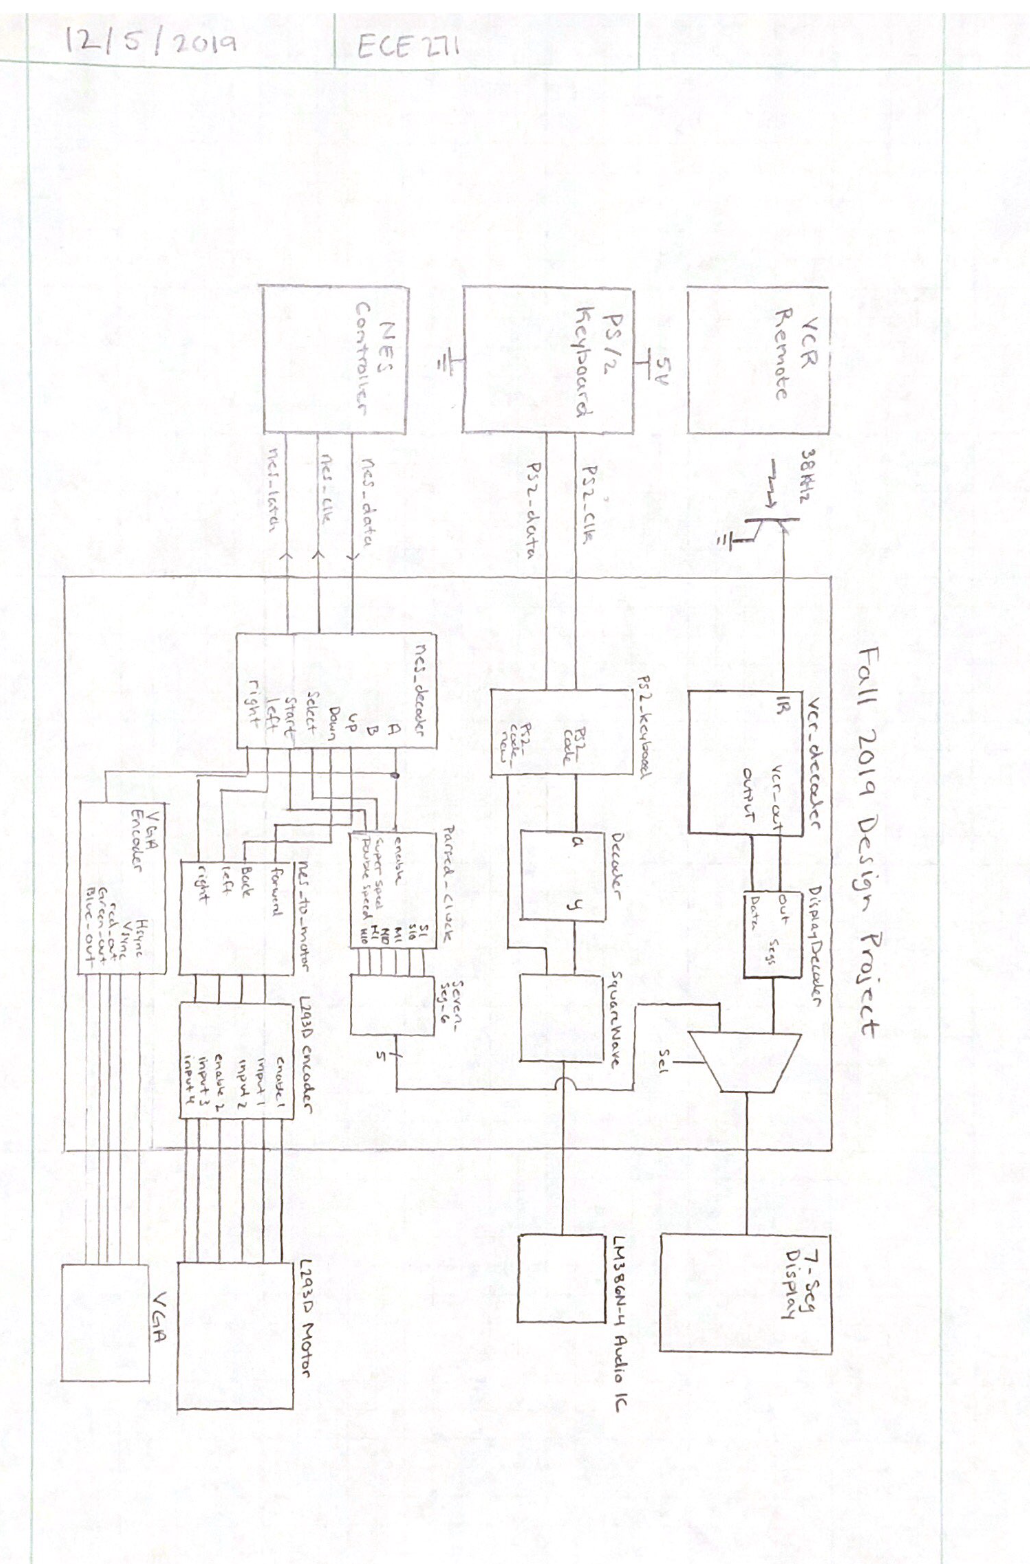
\includegraphics[width=.8\textwidth]{images/project_description.png}
	\caption{Top Level Diagram for the project. The Diagram shows all the Functional Units used in the project and how they are connected from input to output.}
  \label{fig:description}
\end{figure}

\begin{figure}[h]
  \centering
    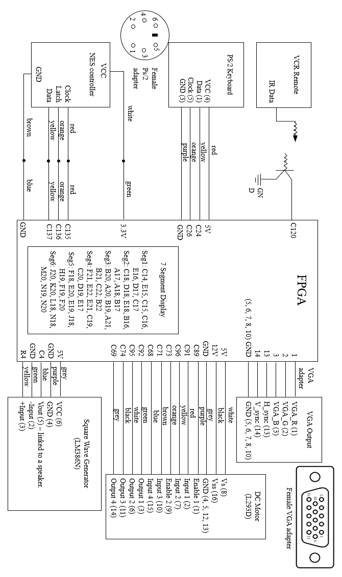
\includegraphics[width=.8\textwidth]{images/hardware_diagram.png}
	\caption{The hardware diagram shows which pins are used on the FPGA, module boards, and relevant supply voltages for the different pieces of hardware used in the system.}
    \label{fig:hardware}
\end{figure}



\clearpage



\section{High Level Description}
This section provides a Top level introduction to the project. The input and output specifications are provided below, as well as a toplevel diagram in \textbf{Figure 3}, and the simulation results in \textbf{Figure 4}.


\begin{itemize}
  \item \textbf{Inputs:  } The Top Level of the project has 7 inputs: switch1, switch2, system\_reset\_button, nes\_data, clock\_50MHz, ps2\_clk, and ps2\_data.
    \begin{itemize}
      \item \textbf{switch1: } switch1 is used to enable the square wave generator unit connected to the PS2 Keyboard.
      \item \textbf{switch2: }
      \item \textbf{system\_reset\_button: } system\_reset\_button is an active high signal used to reset the nes\_decoder, vga\_encoder, and parsed\_clock Functional Units.
      \item \textbf{nes\_data: } the input signal from the NES Controller into the nes\_decoder Functional Unit.
      \item \textbf{clock\_50MHz: } the internal clock on the FPGA that is used generate all the other clock signals used in the top level.
      \item \textbf{ps2\_clk: } the clock signal driving the ps\_2\_keyboard Functional Unit.
      \item \textbf{ps2\_data: } the input signal from the PS2 Keyboard into the ps2\_keyboard functional unit.
    \end{itemize}
  \item \textbf{Outputs: } The Top level has outputs going to the NES Controller, the seven segment pins in the FPGA, the L293D DC Controller, the square wave generator, and the VGA pins.
\end{itemize}

\begin{figure}[h]
  \centering
    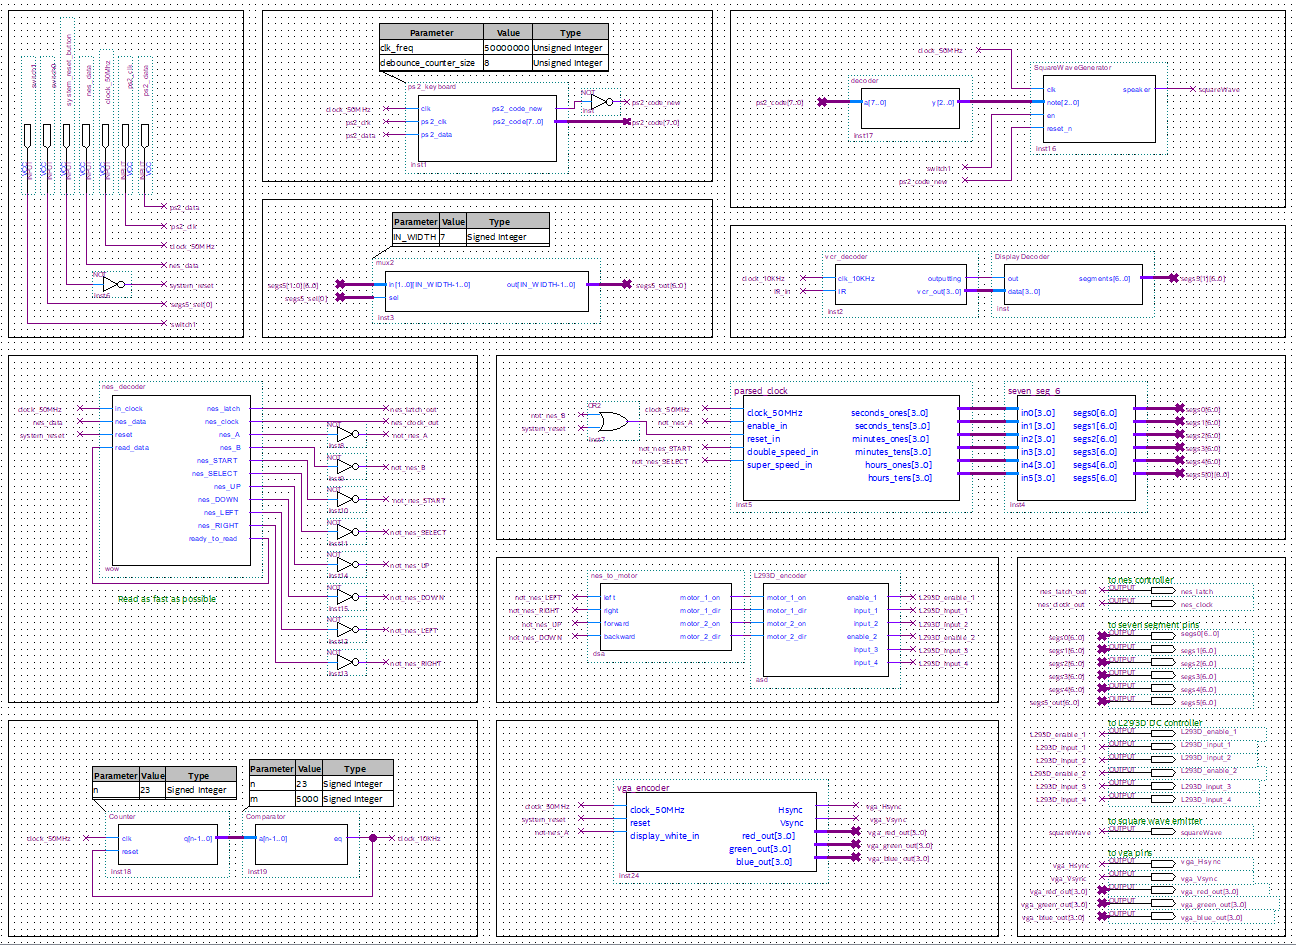
\includegraphics[width=.98\textwidth]{images/top_level.png}
	\caption{The top level design for the  project.}
    \label{fig:top-level}
\end{figure}

\clearpage


\begin{figure}[h]
  \centering
  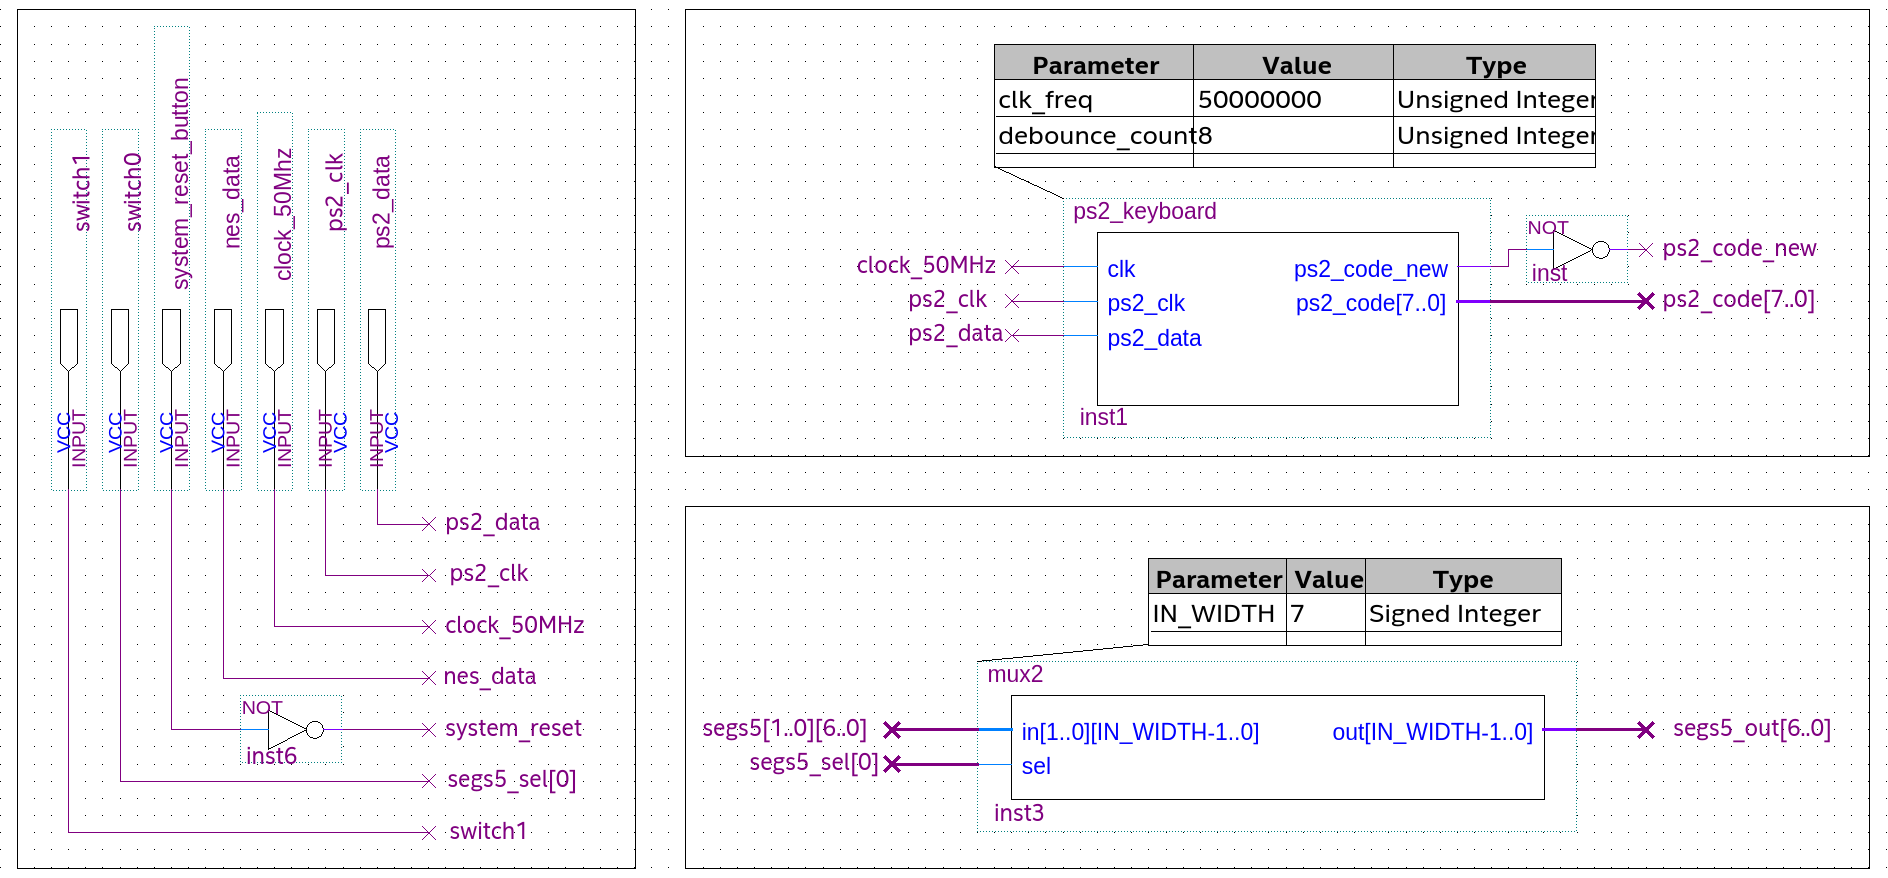
\includegraphics[width=.8\textwidth]{images/top_level_block_1.png}
  \subcaption{Block 1 of top level. Includes the inputs to the Top Level of the design, the ps2\_keyboard Functional unit, and the Multiplexer Functional Unit that controls input to the seven segment display.}
  \label{fig:top-level-block-1}
\end{figure}

\begin{figure}[h]
  \centering
  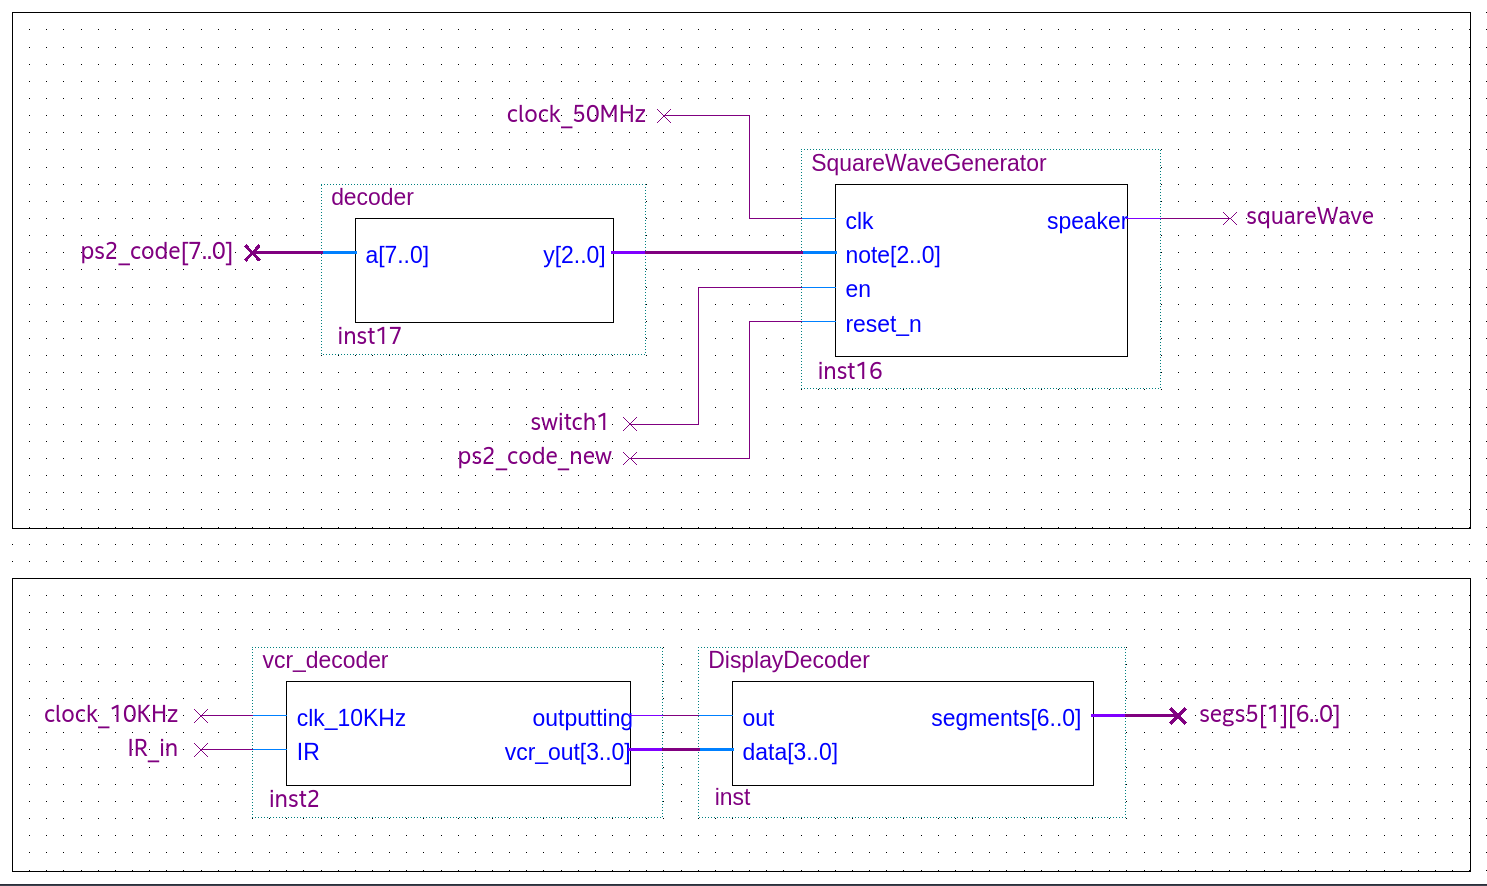
\includegraphics[width=.8\textwidth]{images/top_level_block_2.png}
  \subcaption{Block 2 of top level. Includes the decoder for the ps2\_keyboard functional unit, the square wave generator functional unit, the vcr\_decoder functional unit, and the DislayDecoder functional unit.}
  \label{fig:top-level-block-2}
\end{figure}

\begin{figure}[h]
  \centering
  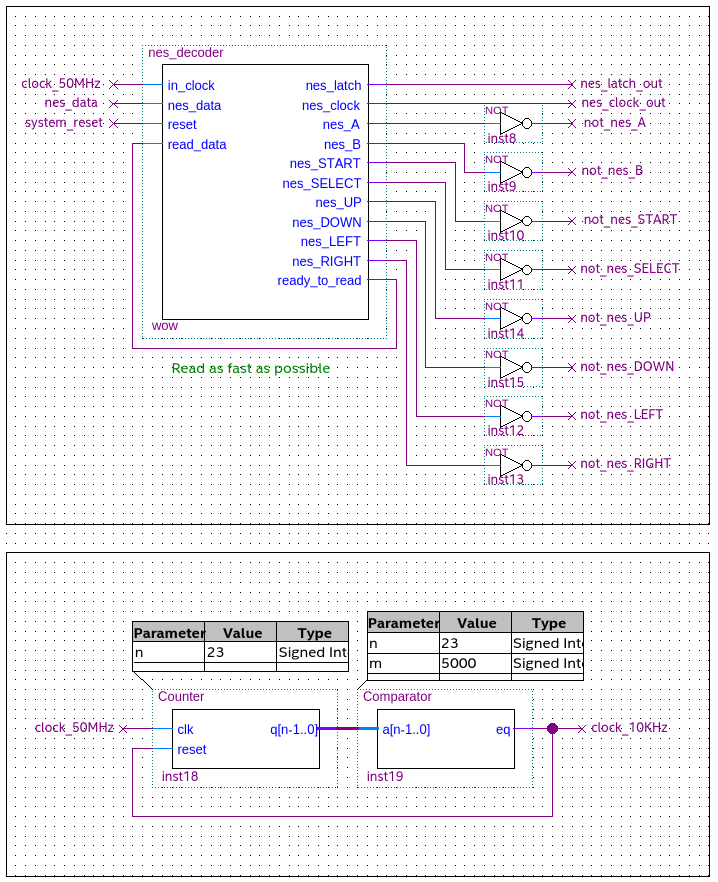
\includegraphics[width=.8\textwidth]{images/top_level_block_3.png}
  \subcaption{Block 3 of top level. Includes the nes\_decoder functional unit and the Counter and Comparator functional units used to generate the clock signal for the vcr\_decoder}
  \label{fig:top-level-block-3}
\end{figure}

\begin{figure}[h]
  \centering
  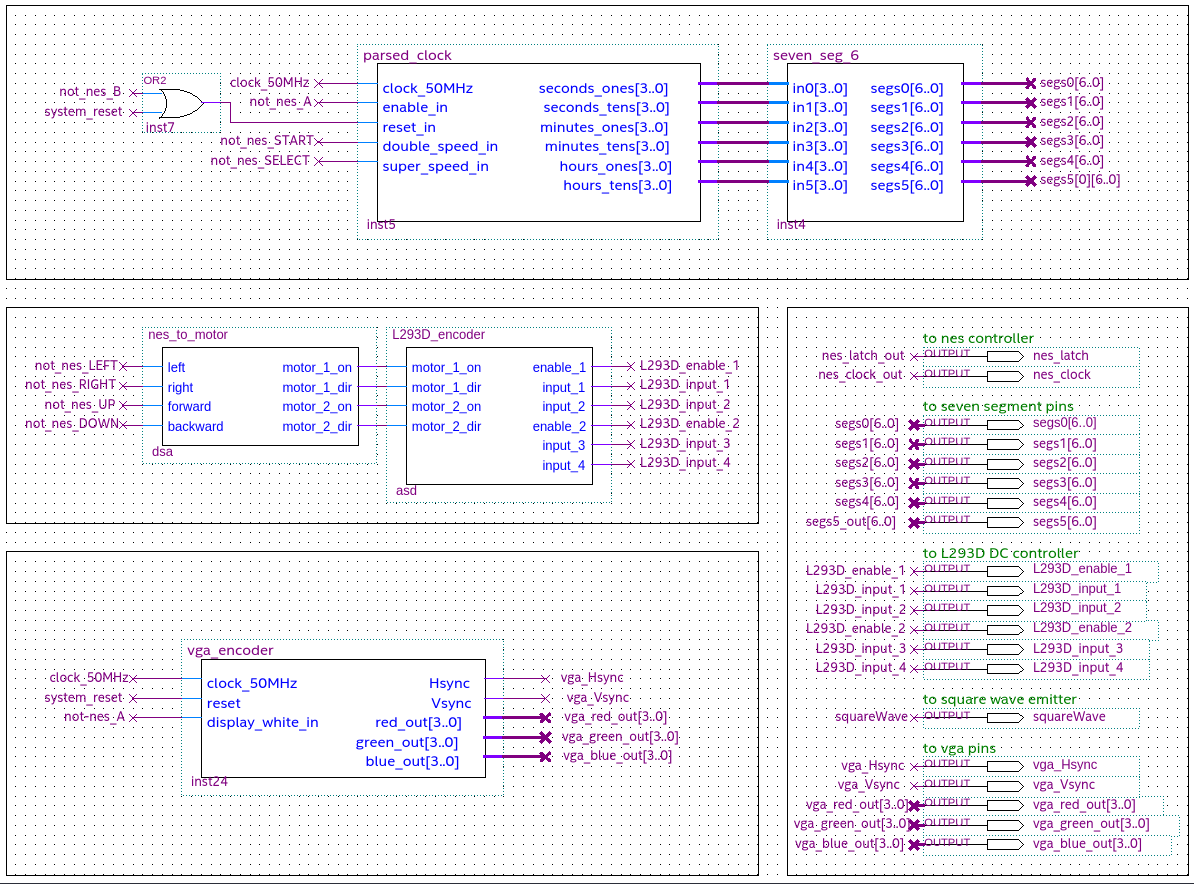
\includegraphics[width=.8\textwidth]{images/top_level_block_4.png}
  \subcaption{Block 4 of top level. Includes the parsed\_clock, seven\_seg\_6, nes\_to\_motor, L293D\_Encoder, and vga\_endocder functional units. In addition, it includes the outputs for the Top Level of the project.}
  \label{fig:top-level-block-4}
\end{figure}


\begin{figure}[h]
  \centering
    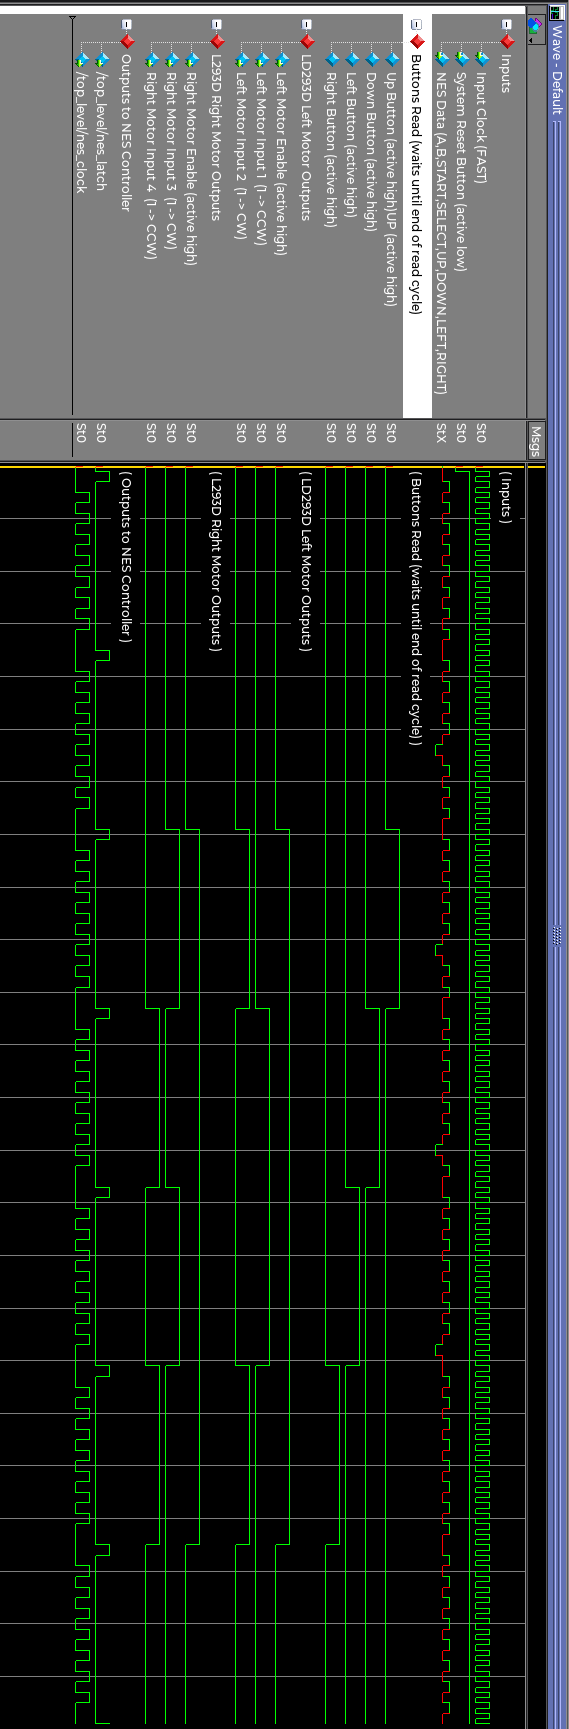
\includegraphics[height=0.98\textheight]{sims/top_level_motor_sim.png}
	\caption{The simulation results for the L293D DC Motor in the Top Level.}
    \label{fig:top-level-sim}
\end{figure}

\begin{figure}[h]
  \centering
    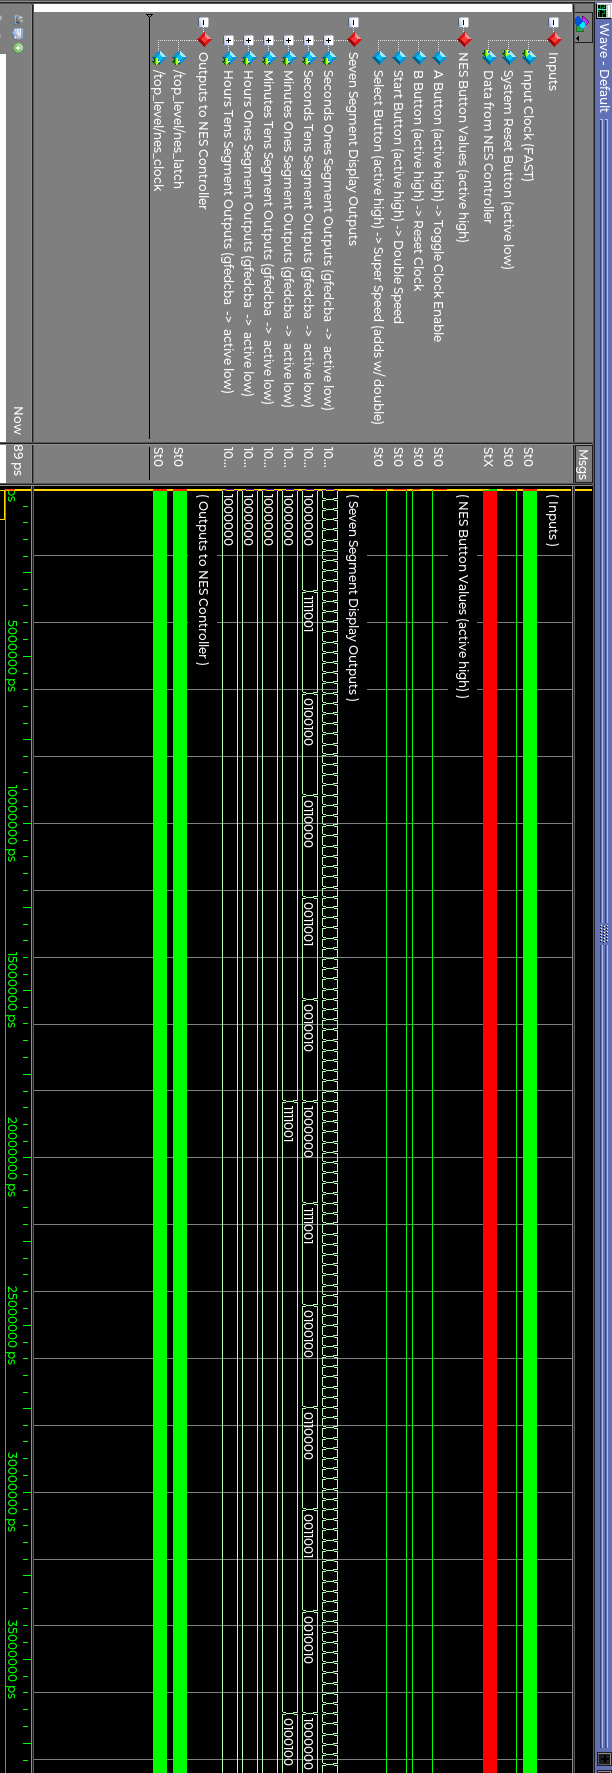
\includegraphics[height=0.98\textheight]{sims/top_level_clock_sim_1.png}
	\caption{The simulation results for the NES Controller to seven segment display in Top Level.}
    \label{fig:top-level-sim}
\end{figure}

\begin{figure}[h]
  \centering
    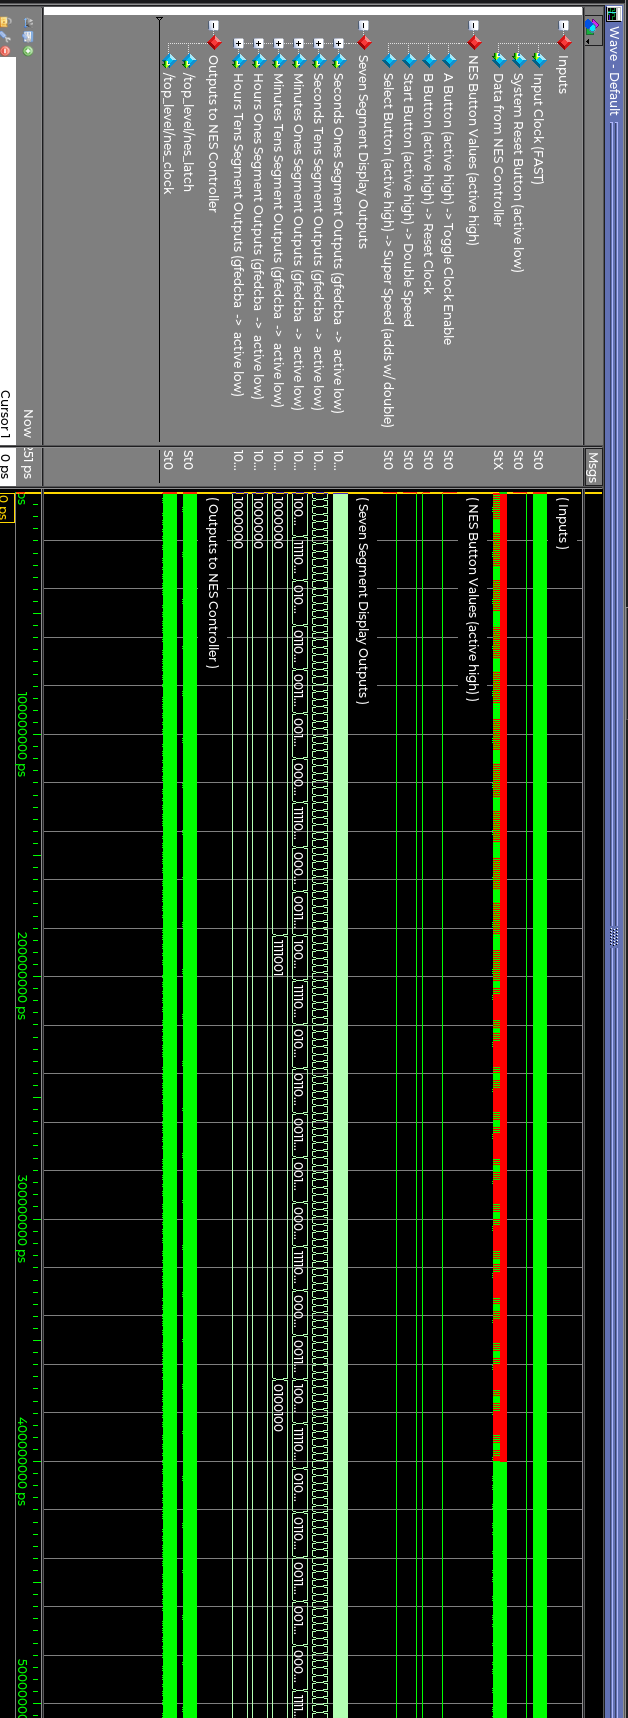
\includegraphics[height=0.98\textheight]{sims/top_level_clock_sim_2.png}
	\caption{The simulation results for the NES Controller to seven segment display in Top Level.}
    \label{fig:top-level-sim}
\end{figure}

\begin{figure}[h]
  \centering
    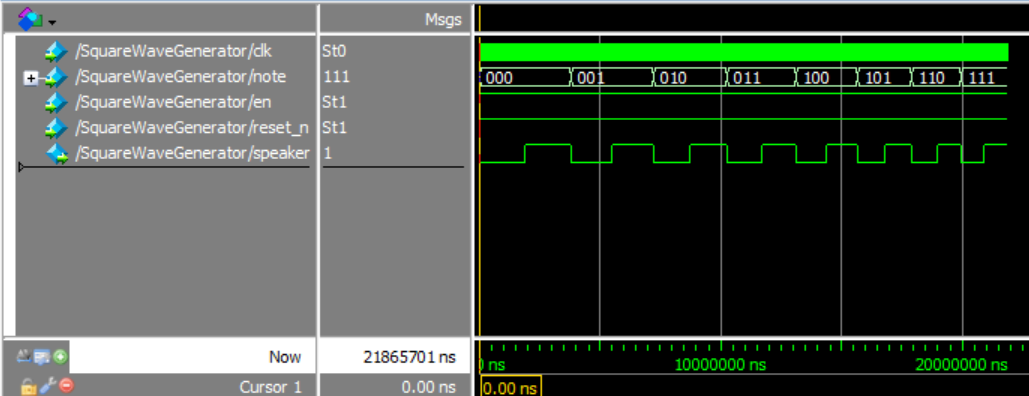
\includegraphics[width=0.98\textwidth]{sims/square_wave_generator/SquareWaveGenerator.png}
	\caption{The simulation results for the PS2 Keyboard to the LM386N-4 Audio IC in Top Level.}
    \label{fig:top-level-sim}
\end{figure}


\begin{figure}[t]
  \centering
  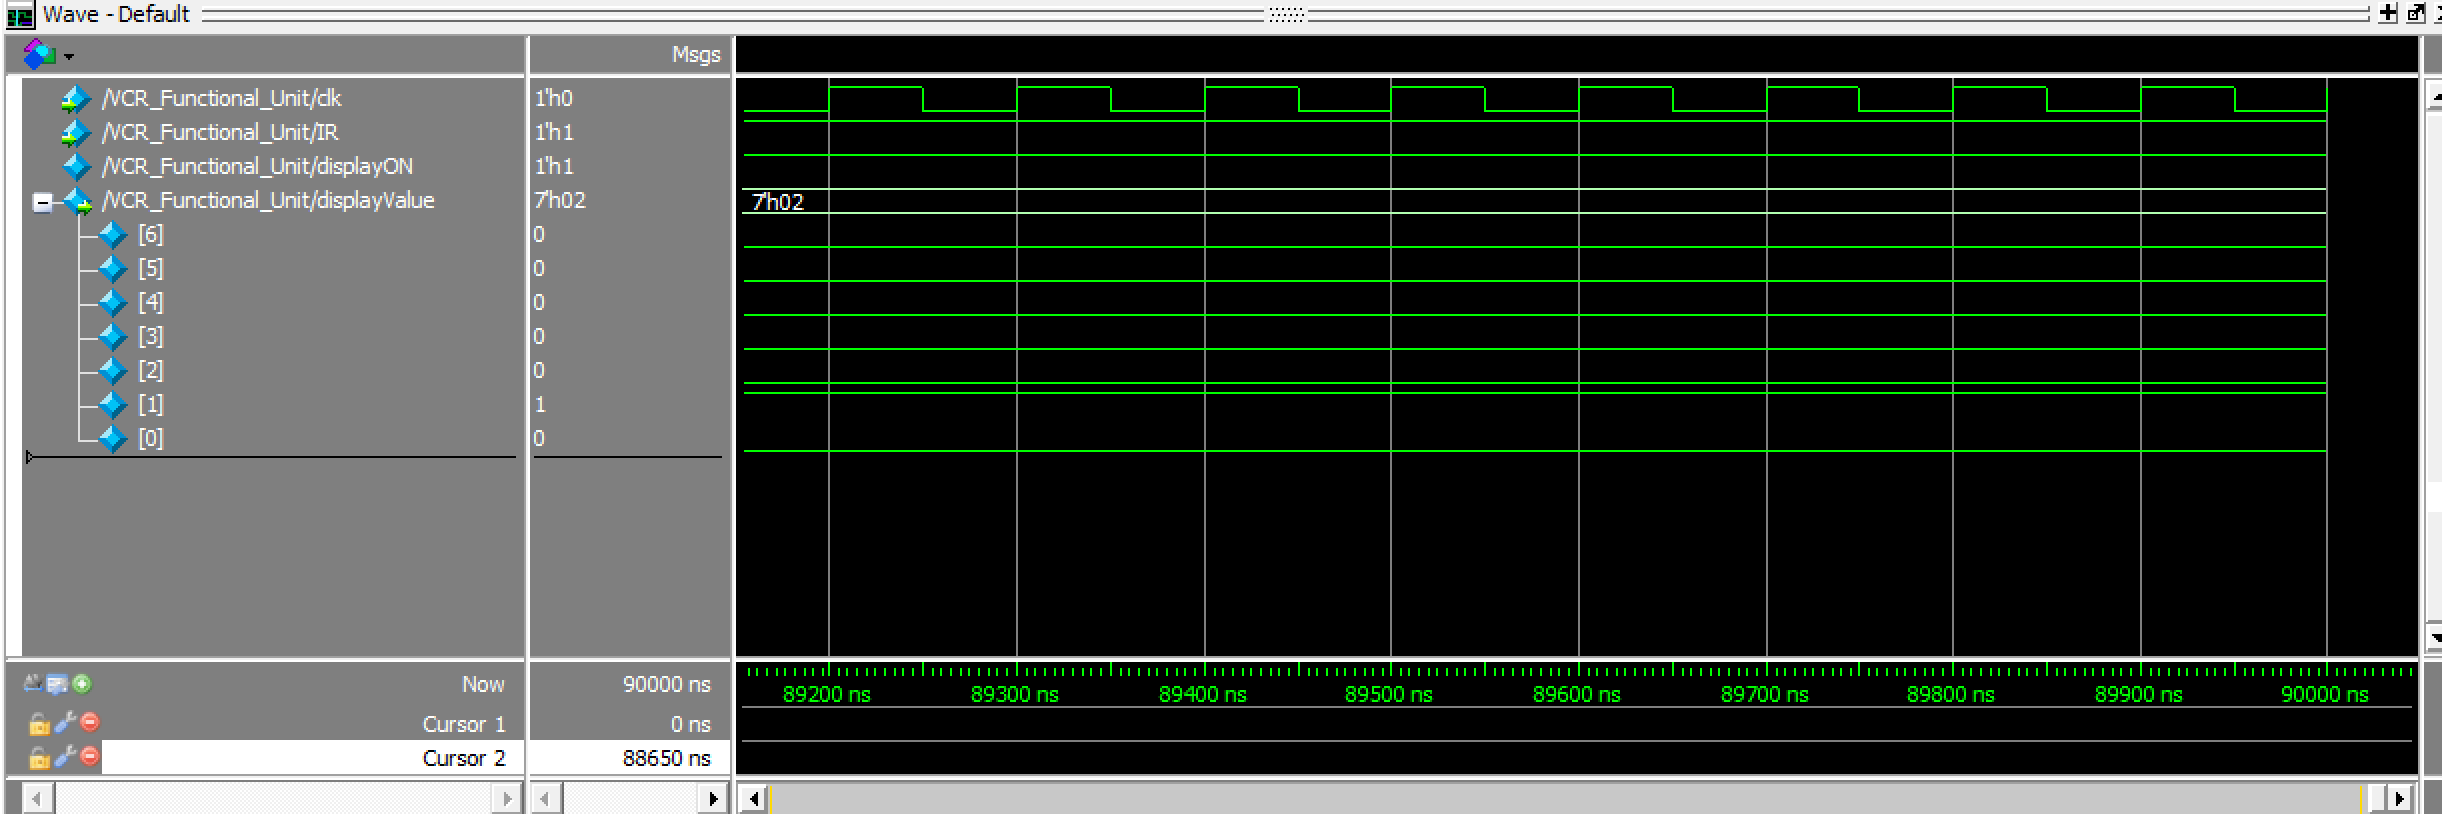
\includegraphics[width=.98\textwidth]{sims/vcr_testing/functionalUnittest/FunctionalUnitTest_6.png}
  \caption{The Simulation results for Top Level VCR output with expected value of 6.}
  \label{fig:top-level-block-1}
\end{figure}

\begin{figure}[t]
  \centering
  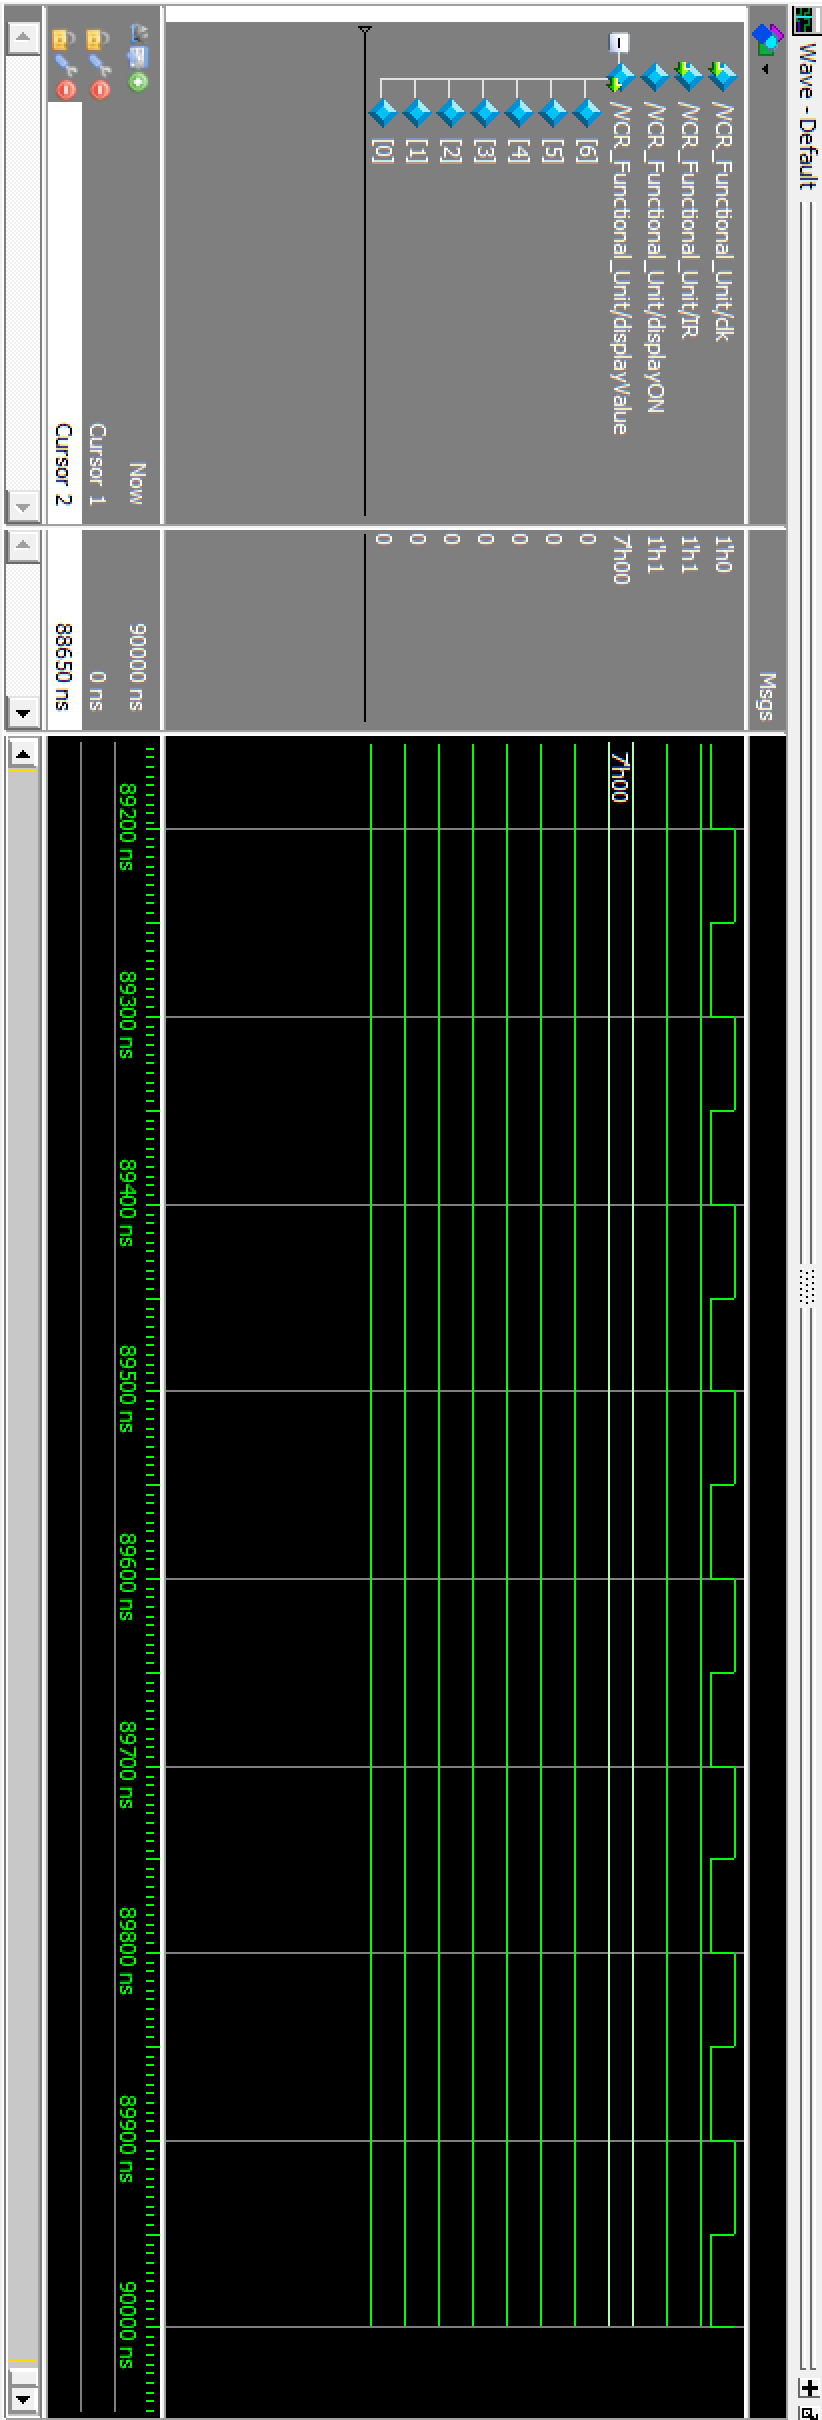
\includegraphics[width=.98\textwidth]{sims/vcr_testing/functionalUnittest/FunctionalUnitTest_8.png}
  \caption{The Simulation results for Top Level VCR output with expected value of 8.}
  \label{fig:top-level-block-1}
\end{figure}


\FloatBarrier

The following subsections will discuss the inputs, outputs, designs, and simulation results of all elements of the design at two levels of scrutiny: functional units and individual blocks of digital logic.



\clearpage


%% Functional Subsections
GENERATE ME




\clearpage



\subsection{DisplaysDecoder Functional Unit}
The DisplayDecoder Module converts a 4-bit input value into a display value on the seven segment display of the FPGA. The DisplayDecoder is
able to output a hexadecimal display value between 0 and F. A block diagram of the unit follows in \textbf{Figure A} and the simulation results for the unit follows in \textbf{Figure B}.
\begin{itemize}
  \item \textbf{Inputs:  } The DisplayDecoder module takes a 4-bit binary value input, data, as its only input.
  \item \textbf{Outputs: } The DisplayDecoder module outputs a 7-bit binary value that is used to activate specific segments in the FPGA seven segment display.
\end{itemize}
\begin{figure}[h]
  \centering
    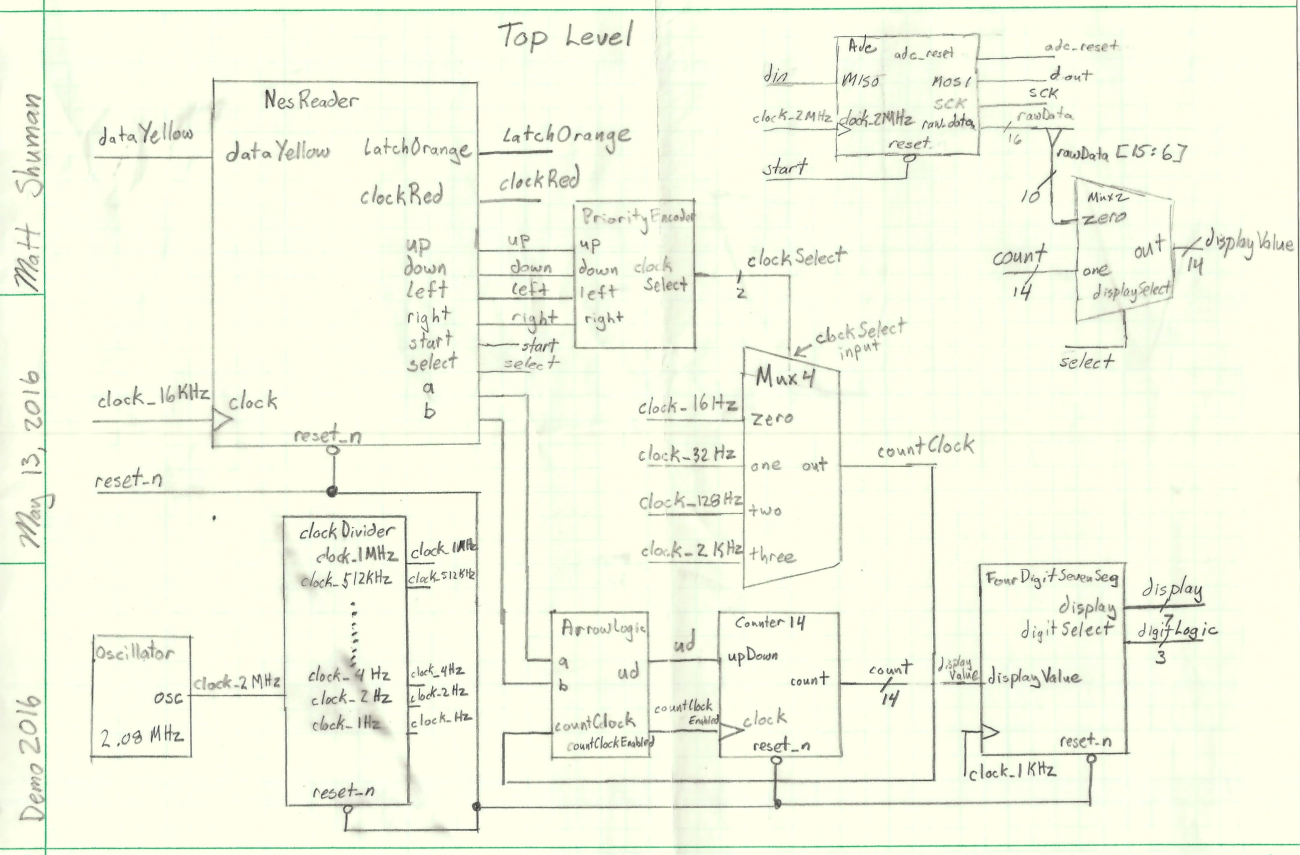
\includegraphics[width=.8\textwidth]{images/functional_1.png}
	\caption{The logic design of the DisplayDecoder functional unit used in the final design.}
    \label{fig:functional-1}
\end{figure}
\begin{figure}[h]
  \centering
    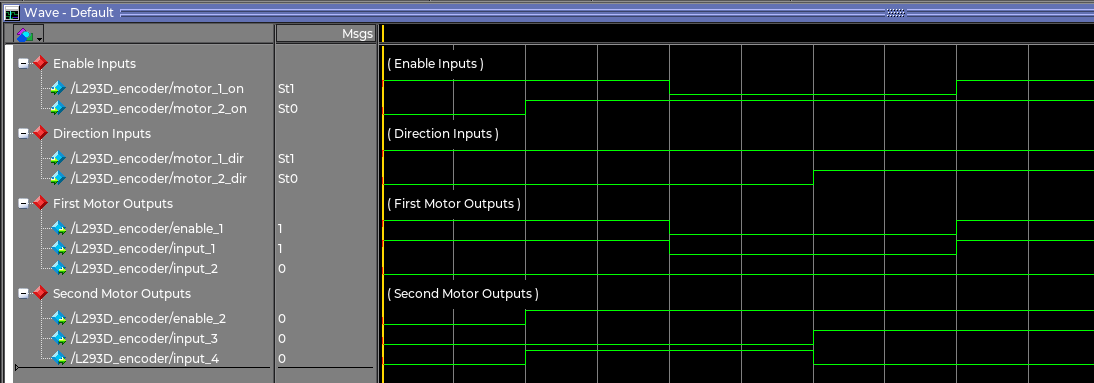
\includegraphics[width=.98\textwidth]{sims/functional_1.png}
	\caption{The simulation results for the DisplayDecoder Individual Unit.}
    \label{fig:top-level-sim}
\end{figure}



\clearpage



\subsection{vcr\_decoder Functional Unit}
The vcr\_decoder module converts an IR signal sent from a VCR remote into a decimal value between 0 and 9. A block diagram of the unit follows in \textbf{Figure A}. A state diagram describing the unit as well as the simulation results for the unit follow in \textbf{Figure B}, and the details for each individual block comprising the unit follow after.
\subsection{vcr decoder Functional Unit}
The vcr\_decoder module converts an IR signal sent from a VCR remote into a decimal value between 0 and 9. A block diagram of the unit follows in \textbf{Figure A}, the simulation results for the unit follows in \textbf{Figure B}, and the details for each individual block comprising the unit follow after.
\begin{itemize}
  \item \textbf{Inputs:  } The vcr\_decoder module two inputs, clk and IR. clk is a 10 KHz clock signal that is used to drive the module. IR is the Infrared signal coming from the VCR remote that will be translated by the module.
  \item \textbf{Outputs: } The vcr\_decoder module has a single output, displayValue, which is the 0-9 representing the IR signal that was received by the module as input.
\end{itemize}
\begin{figure}[h]
  \centering
    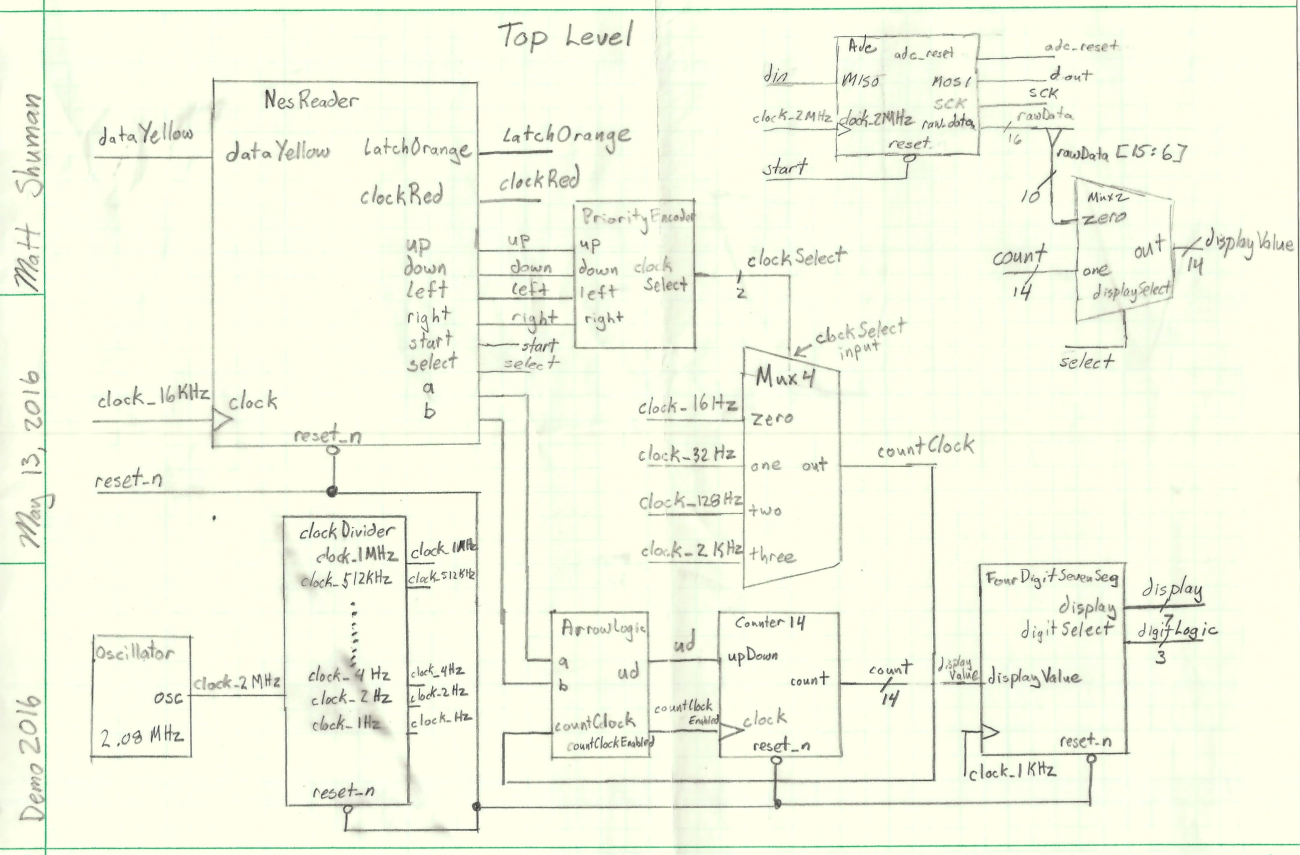
\includegraphics[width=.8\textwidth]{images/functional_1.png}
	\caption{The logic design of the vcr\_decoder functional unit used in the final design.}
    \label{fig:functional-1}
\end{figure}
\begin{figure}[h]
  \centering
    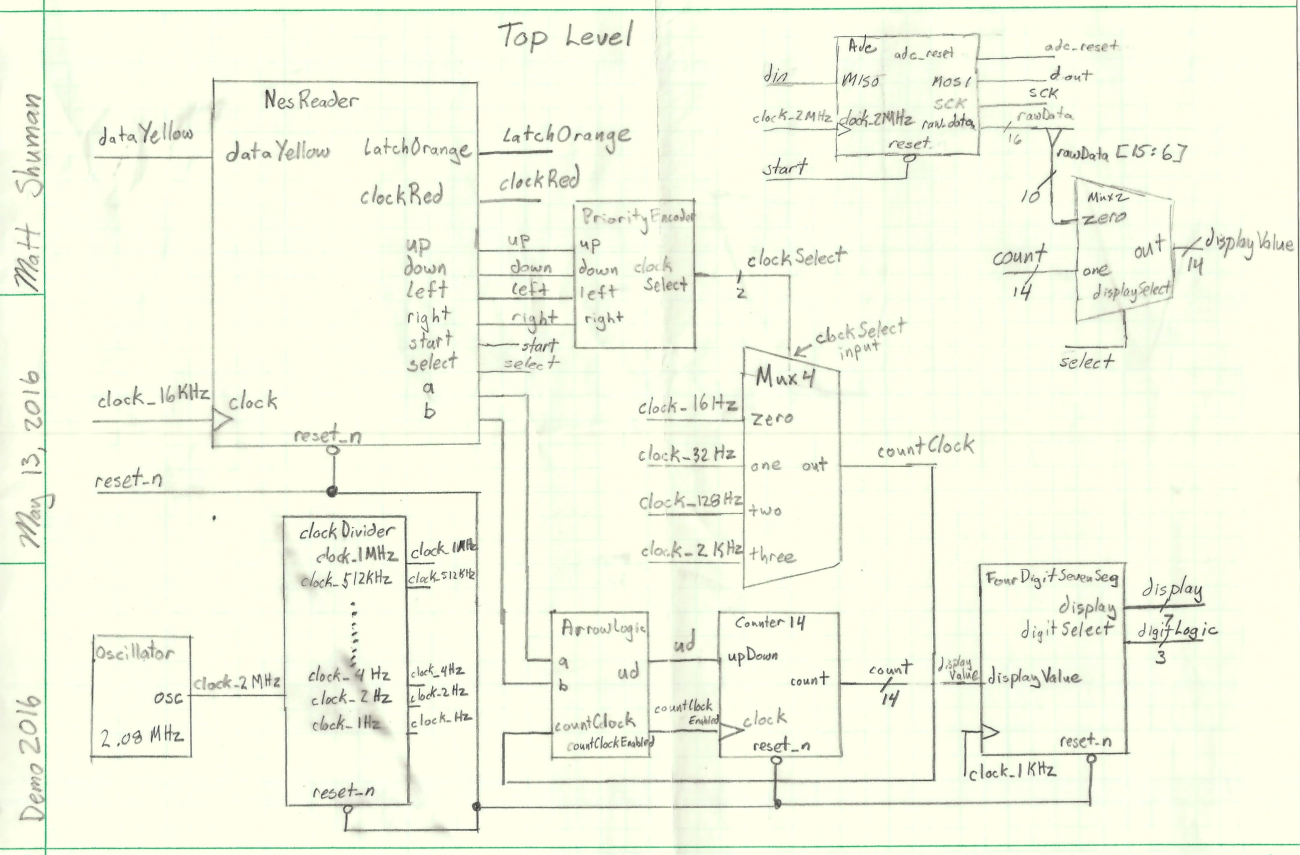
\includegraphics[width=.8\textwidth]{images/functional_1.png}
	\caption{The State Diagram for the vcr\_decoder functional unit used in the final design.}
    \label{fig:functional-1}
\end{figure}
\begin{figure}[h]
  \centering
    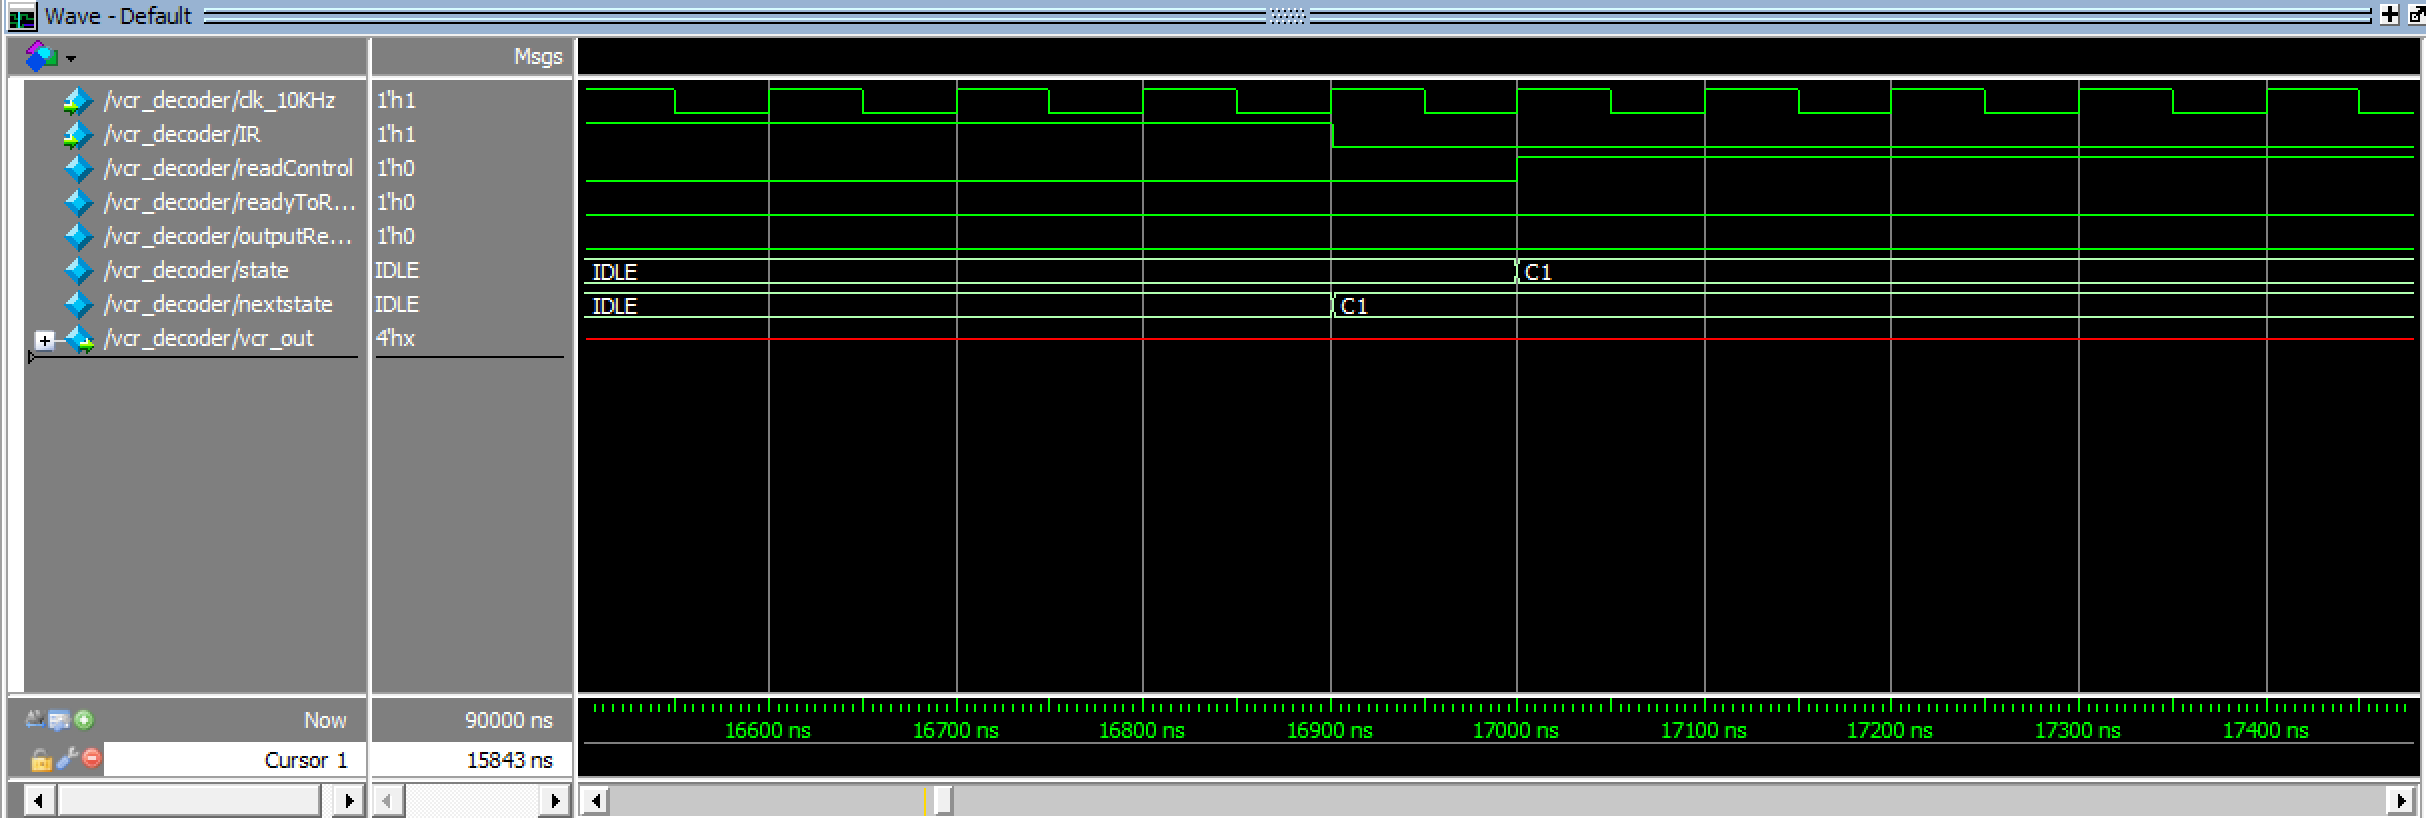
\includegraphics[width=.98\textwidth]{sims/vcr_testing/moduleTests/vcr_decoder/IDLE_to_C1_Transition.png}
	\caption{Simulation results of the vcr\_decoder Functional Unit showing the state transition from the IDLE state to the C1 control state following the first time the IR signal goes to a logic LOW.}
    \label{fig:top-level-sim}
\end{figure}
\begin{figure}[h]
  \centering
    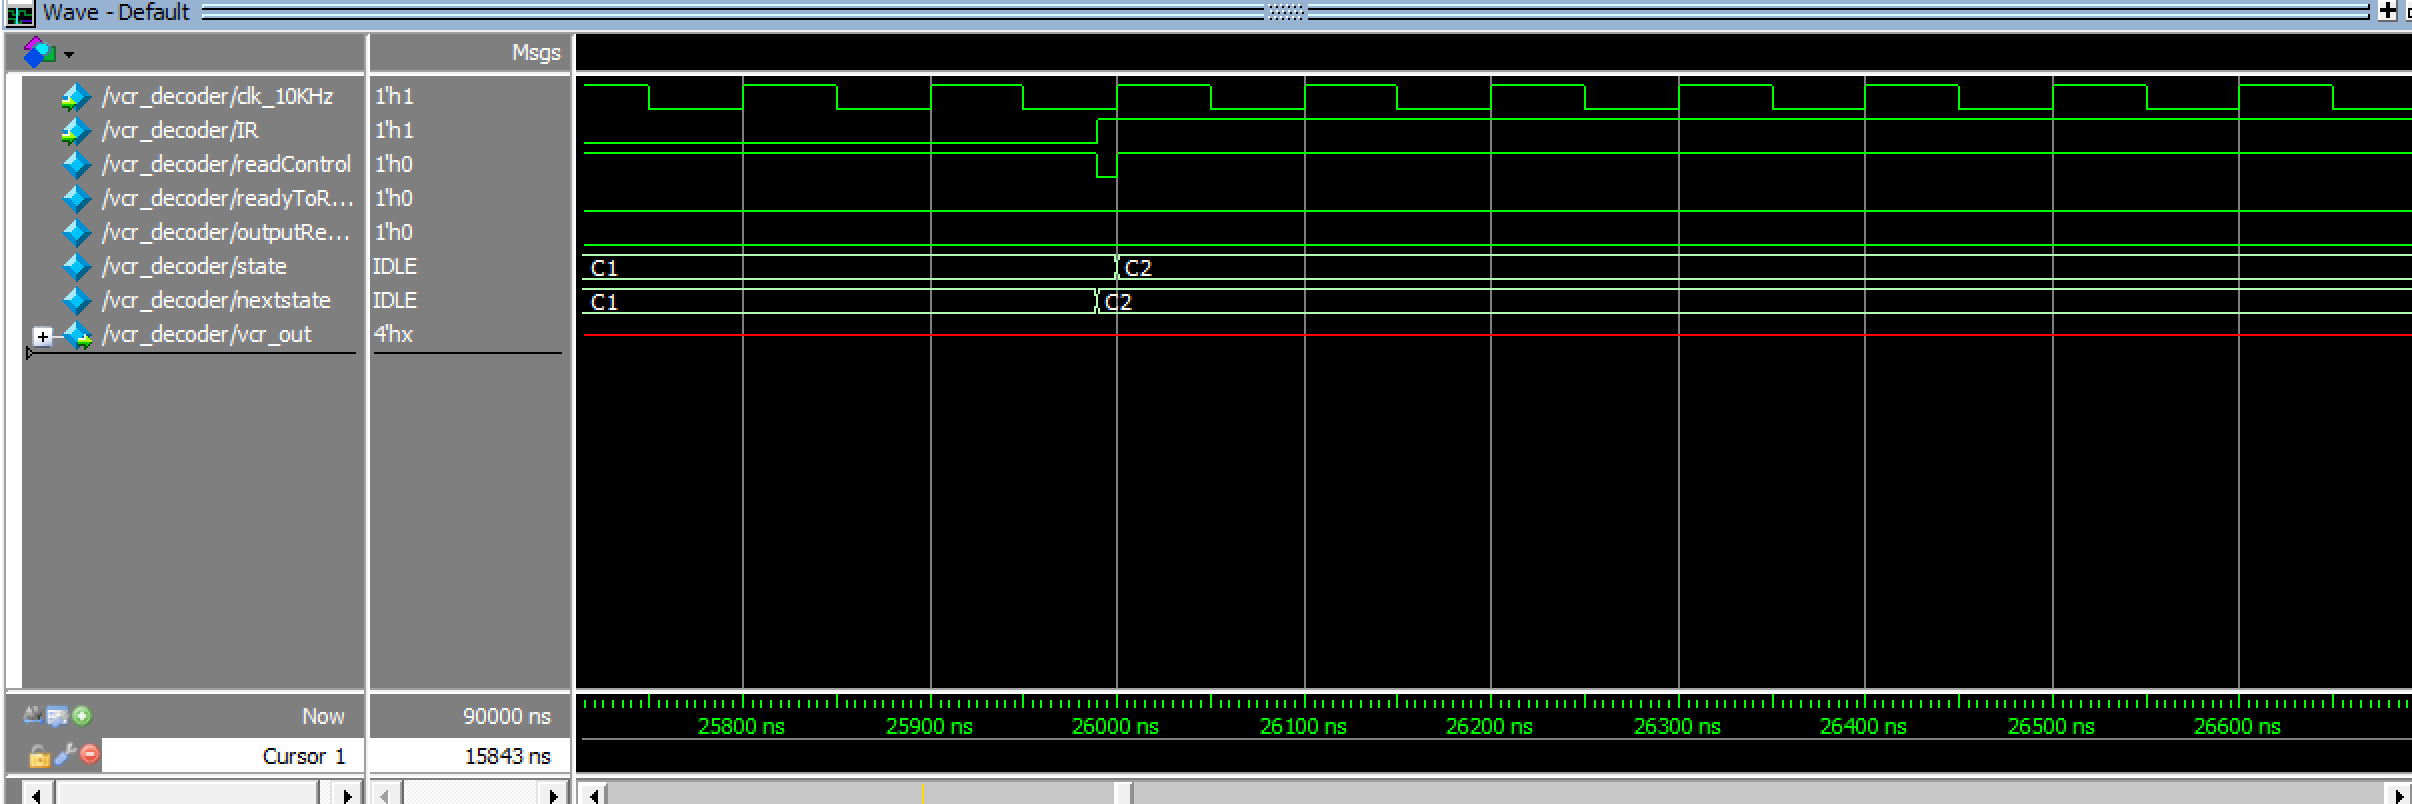
\includegraphics[width=.98\textwidth]{sims/vcr_testing/moduleTests/vcr_decoder/C1_to_C2_transition.png}
	\caption{Simulation results of the vcr\_decoder Functional Unit showing the state transition from the C1 control state to the C2 control state.}
    \label{fig:top-level-sim}
\end{figure}
\begin{figure}[h]
  \centering
    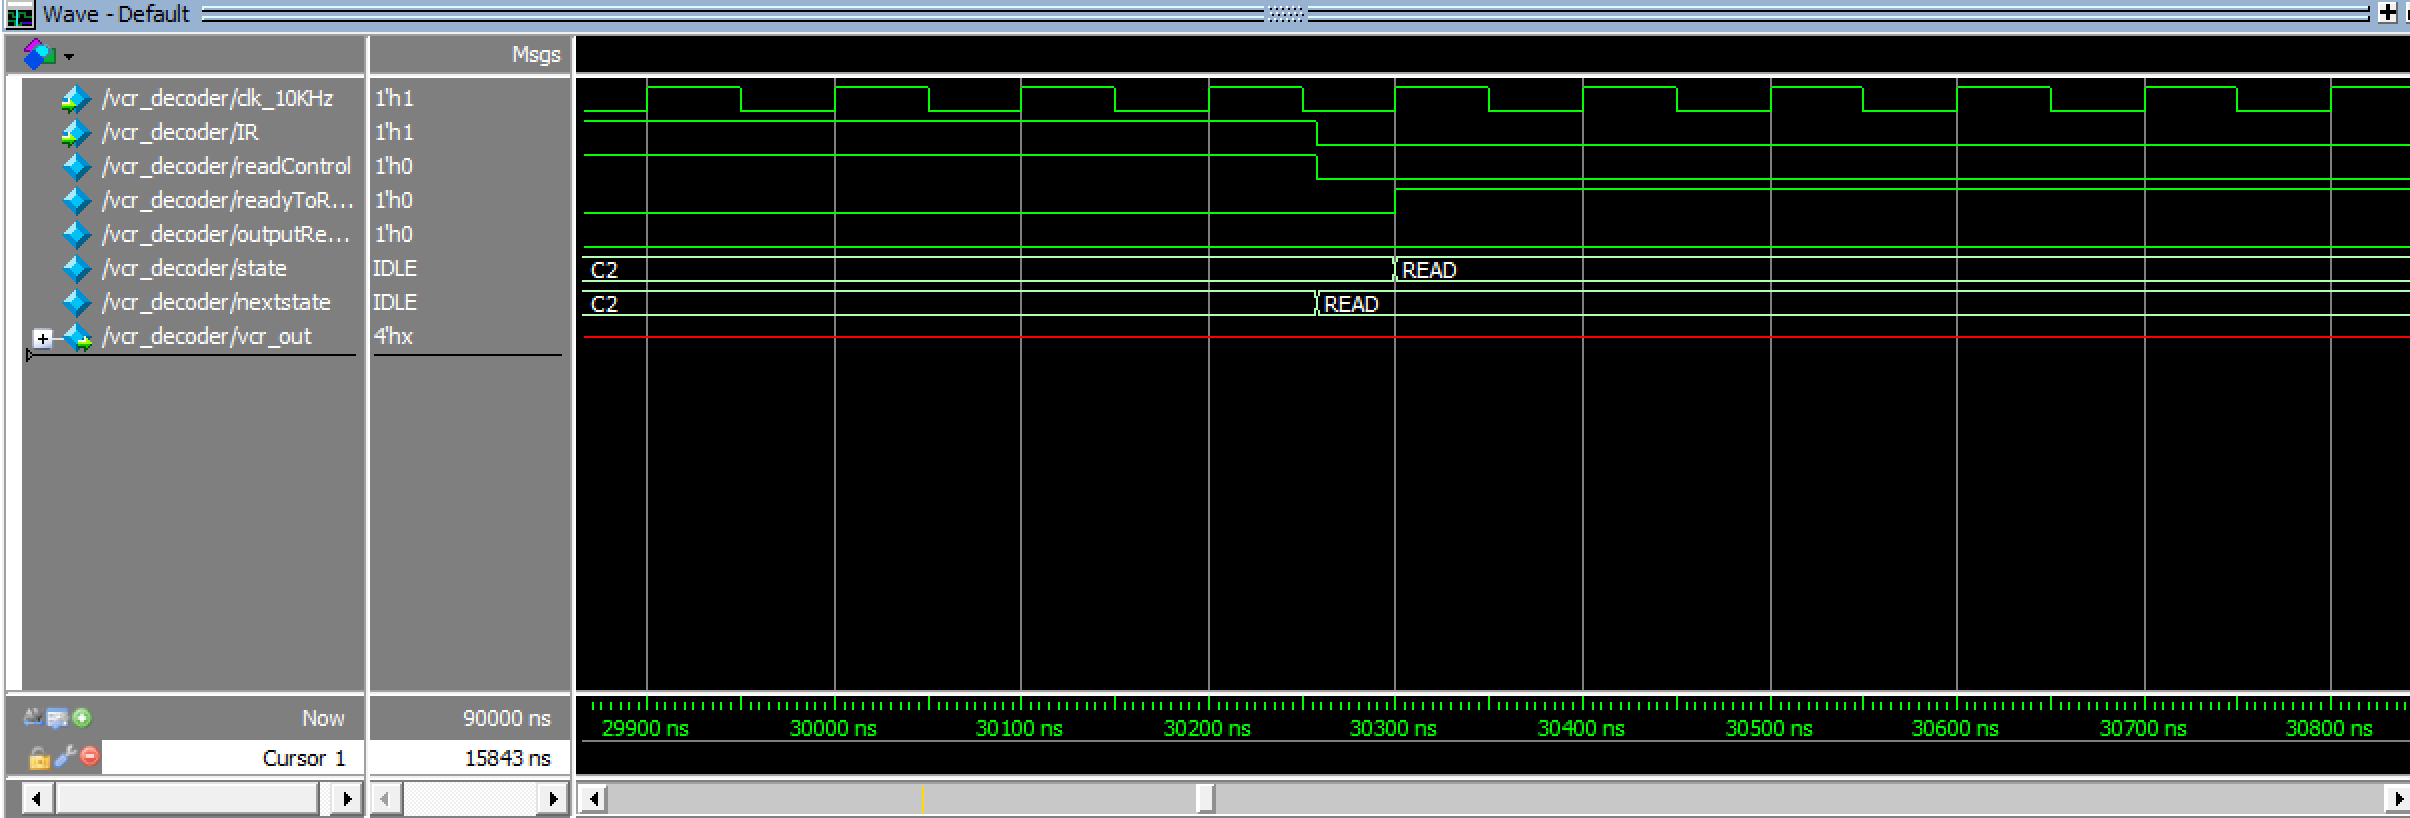
\includegraphics[width=.98\textwidth]{sims/vcr_testing/moduleTests/vcr_decoder/C2_to_READ_transition.png}
	\caption{Simulation results of the vcr\_decoder Functional Unit showing the transition from the C2 control state to the READ state, indicicating that it is currently reading a 32-bit IR signal corresponding the button on the VCR remote that was pressed.}
    \label{fig:top-level-sim}
\end{figure}
\begin{figure}[h]
  \centering
    \includegraphics[width=.98\textwidth]{sims/vcr_testing/moduleTests/vcr_decoder/READ_to_PUSH_transition.png}
	\caption{Simulation results of the vcr\_decoder Functional Unit showing the transition from the READ state to the PUSH state indicating that the full 32-bit input value has been processed and an output value is produced.}
    \label{fig:top-level-sim}
\end{figure}




\clearpage



\subsubsection{ReadState Individual Block}
The ReadState Individual Block is used to implement the READ state within the vcr\_decoder Module. The block diagram (\textbf{Figure C}), State Diagram, and simulation results \textbf{Figure D} are provided below.
\begin{itemize}
  \item \textbf{Inputs:  } inputs
  \item \textbf{Outputs: } outputs
\end{itemize}
\begin{figure}[h]
  \centering
  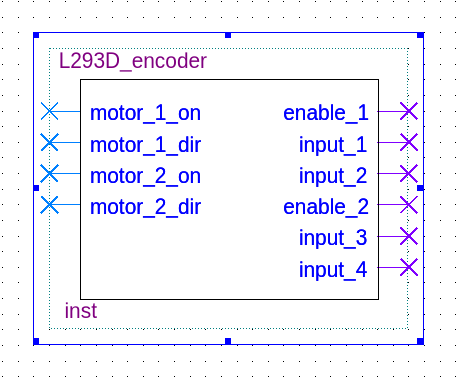
\includegraphics[width=.48\textwidth]{symbols/individual_placeholder.png}
  \caption{The block symbol of the ReadState individual block used in the vcr\_decoder functional unit.}
    \label{fig:individual-1-2-block}
\end{figure}
\begin{figure}[h]
  \centering
  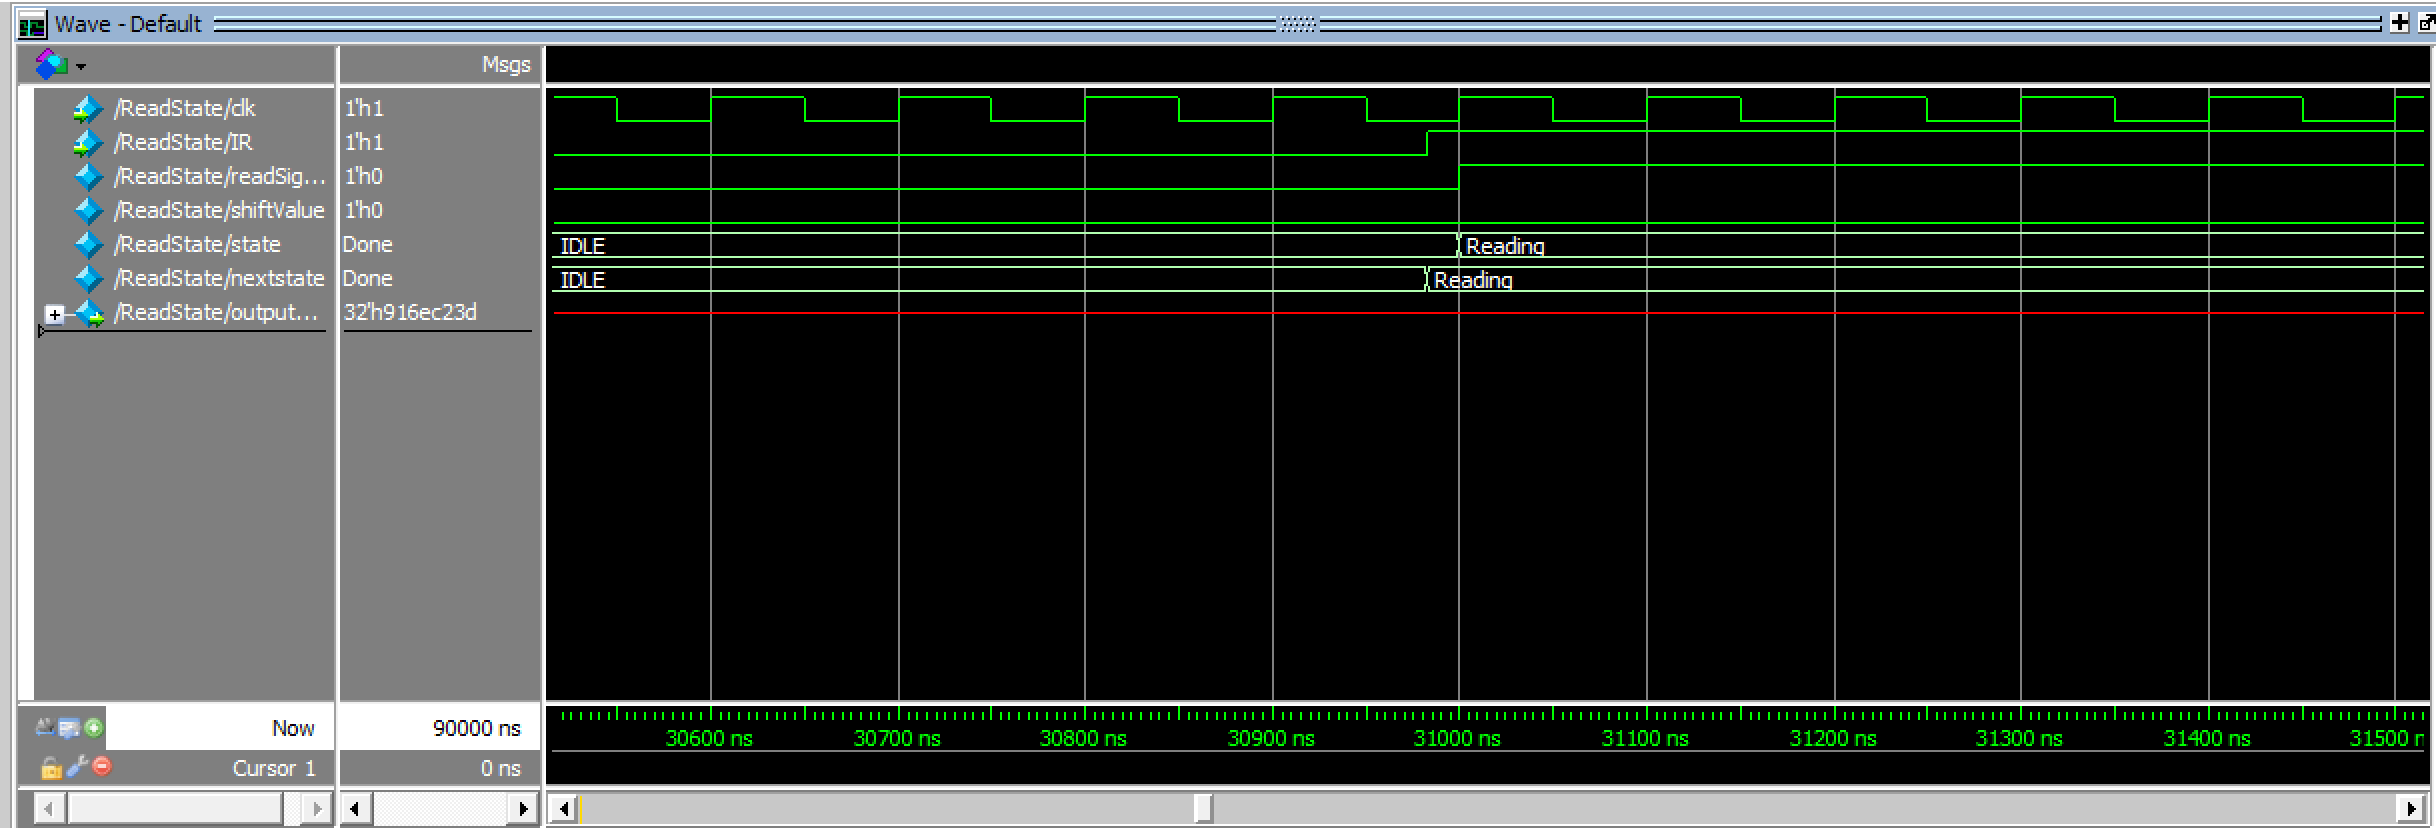
\includegraphics[width=.98\textwidth]{sims/vcr_testing/moduleTests/ReadState/IDLE_to_READING_Transition.png}
  \caption{Simulation results of the ReadState individual block used in the vcr\_decoder functional unit. The simulation shows the transition from the IDLE state to the Reading State within the ReadState Module. This transition is in response to the initial HIGH IR signal that represents the 32-bit value encoding the button that was pressed.}
    \label{fig:individual-1-2-sim}
\end{figure}
\begin{figure}[h]
  \centering
  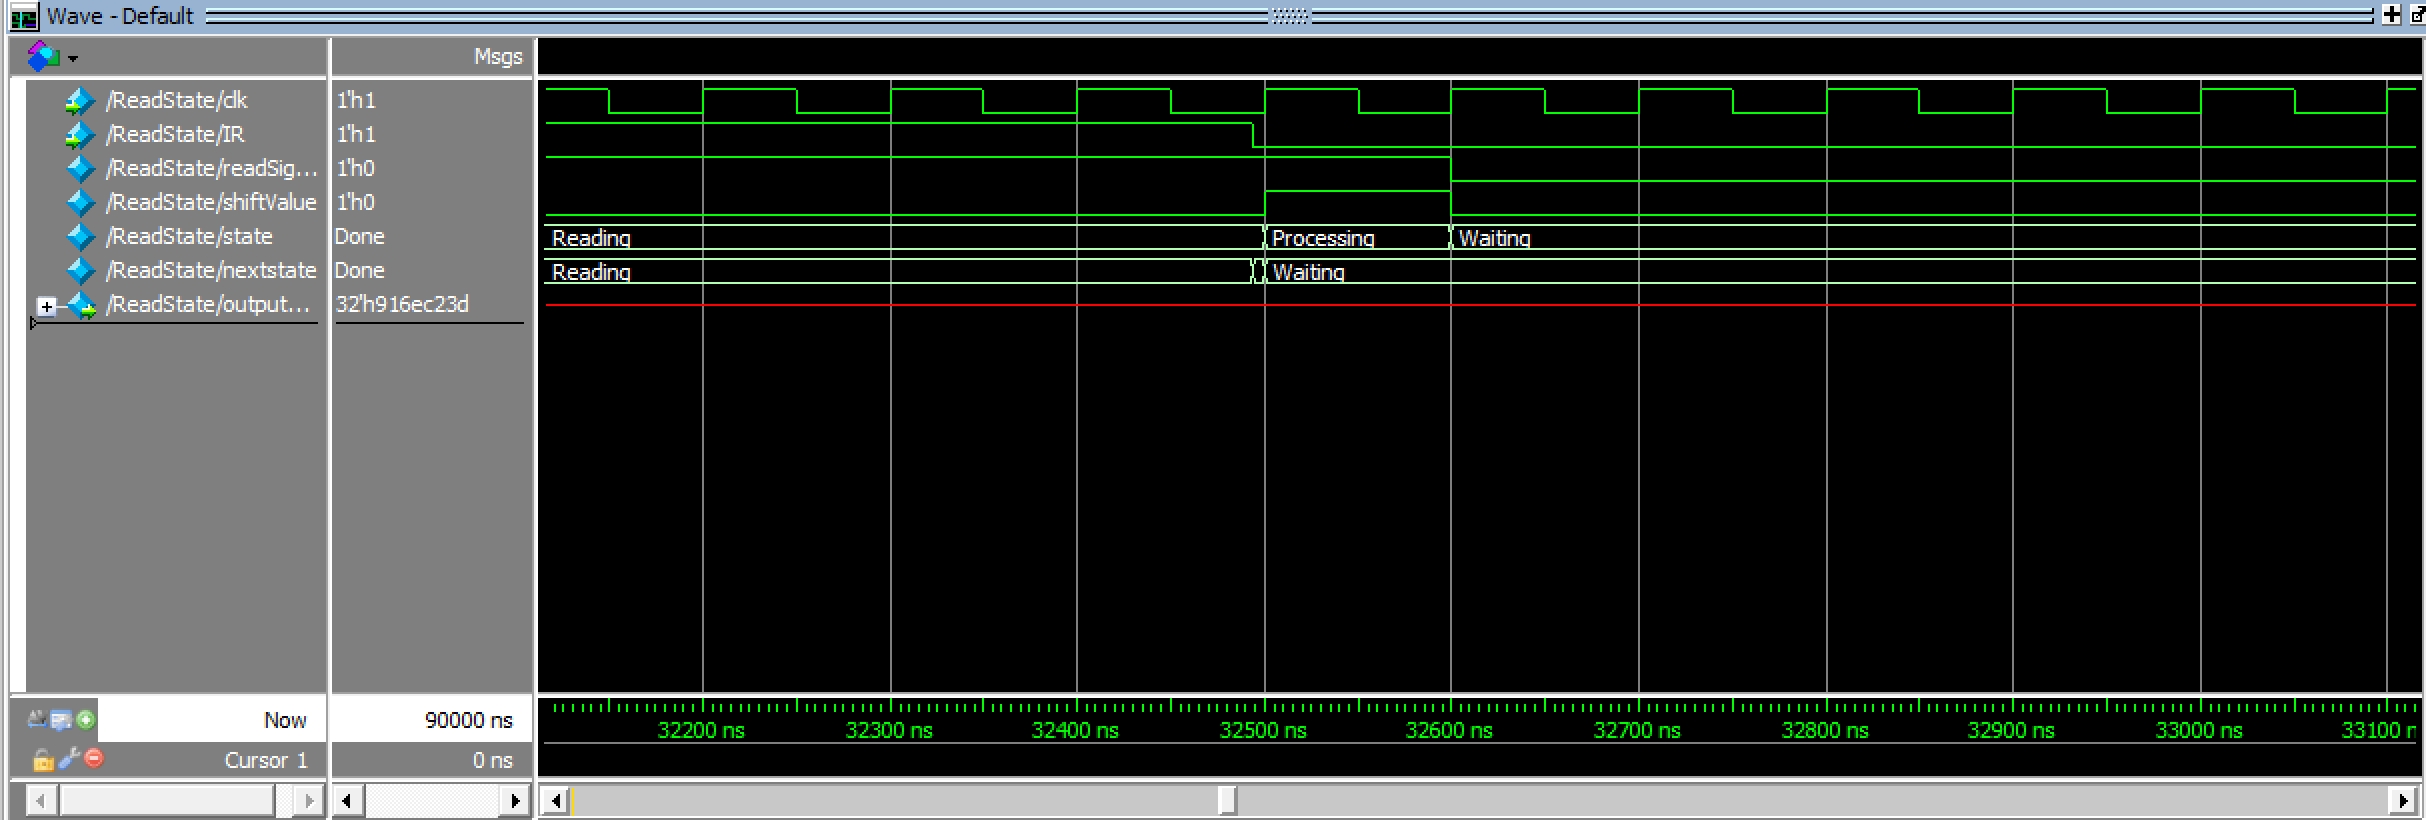
\includegraphics[width=.98\textwidth]{sims/vcr_testing/moduleTests/ReadState/PROCESSING_State.png}
  \caption{Simulation results of the ReadState individual block used in the vcr\_decoder functional unit. The simulation shows Processing State of the ReadState Module. When the state machine is in the Reading state, that means it is actively reading a HIGH signal for IR. As seen in this waveform, when IR goes LOW again, the state machine switches to the Processing state in which it checks the length of the signal to see if it is a logic 1 or a logic 0. The 1 or 0 is then shifted into the shift register on the rising edge of the shiftValue signal, as seen in the waveform. The state machine then switches into the Waiting state, while it waits for IR to go HIGH again.}
    \label{fig:individual-1-2-sim}
\end{figure}
\begin{figure}[h]
  \centering
  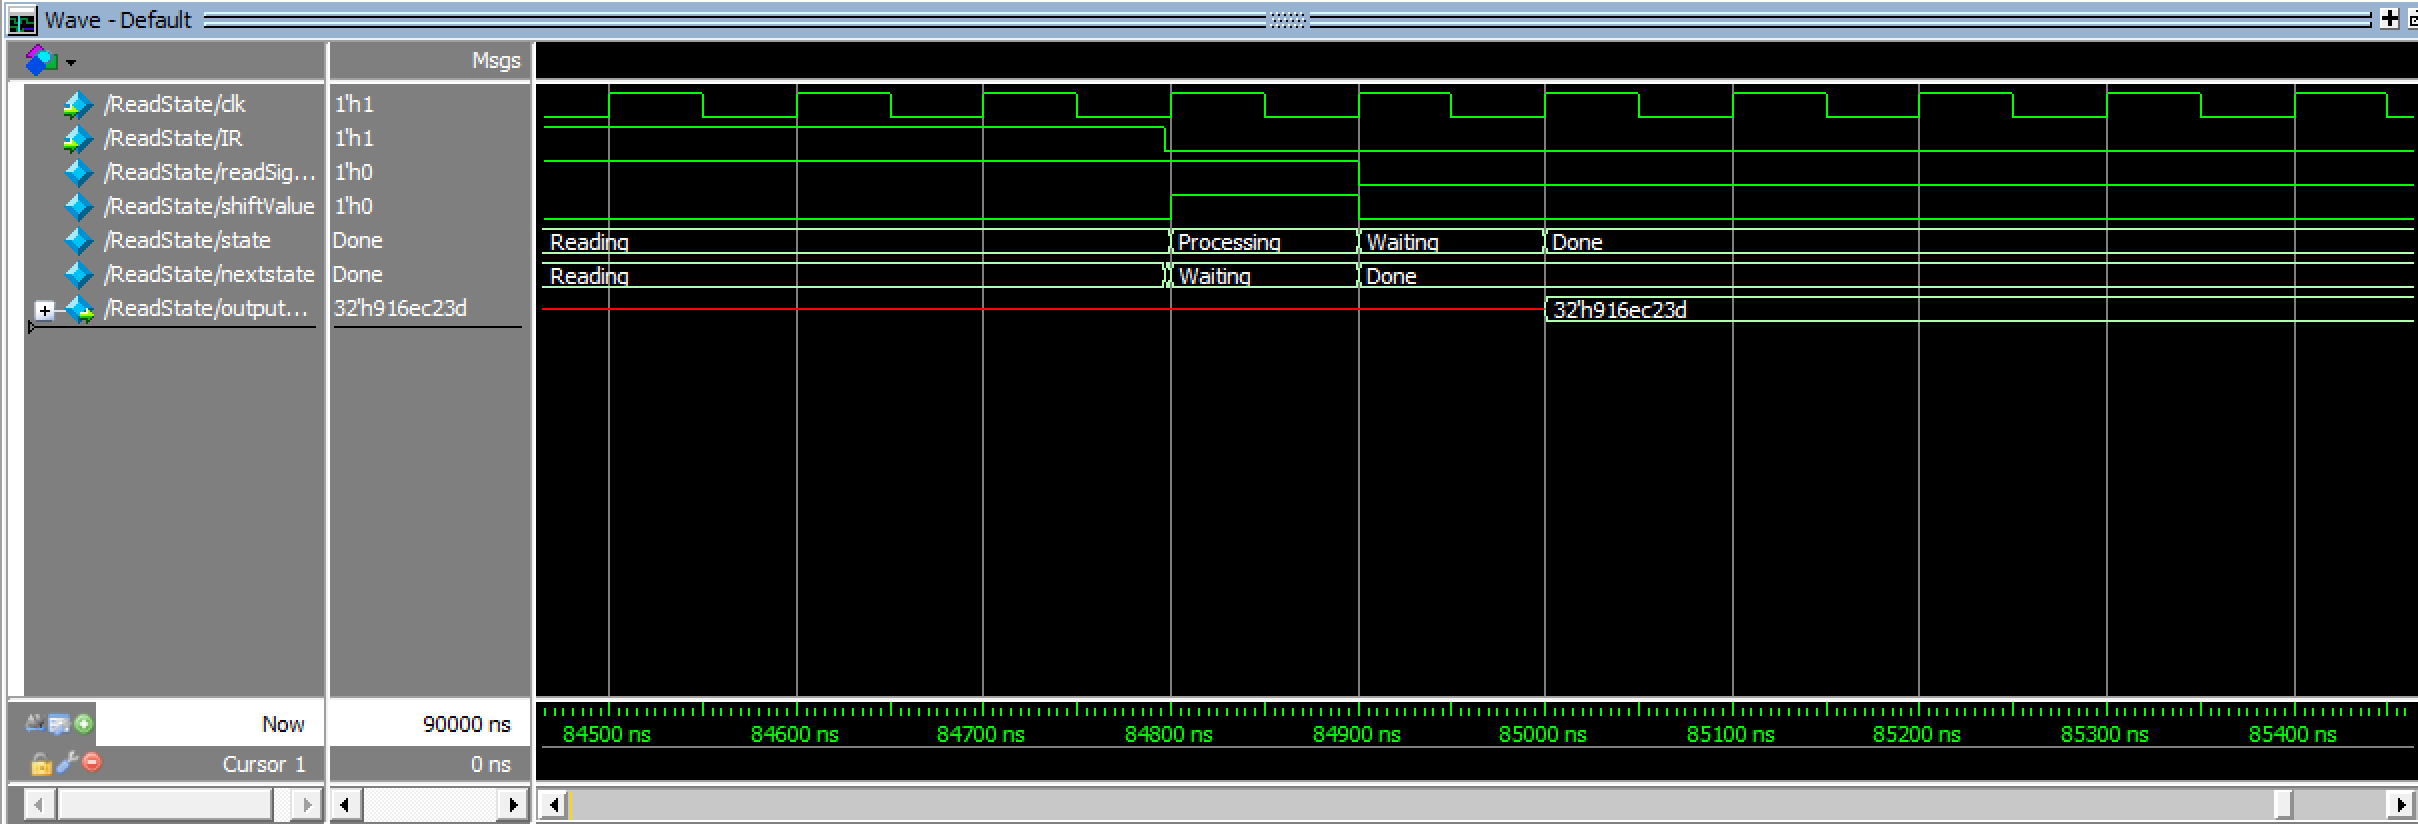
\includegraphics[width=.98\textwidth]{sims/vcr_testing/moduleTests/ReadState/Transition_to_DONE.png}
  \caption{Simulation results of the ReadState individual block used in the vcr\_decoder functional unit. The simulation shows the transition from the reading, Processing, Waiting cycle to the Done state in which it outputs the 32-bit hexadecimal value identified by the IR signal input. In each Waiting state, the state machine will check if 32-bits have been read into the shift register. If so, the state machine will switch to the Done state and output the value for the IR signal that it received as input. In addition, it will drive an output signal outputReady HIGH. This signal is used by the vcr\_decoder module, to know when to output a result.}
    \label{fig:individual-1-2-sim}
\end{figure}



\clearpage



\subsubsection{SignalDecoder Individual Block}
The SignalDecoder Individual Block is used to convert the 32-bit value generated by the ReadState Individual Block into a 4-bit value by 0 and 15 that indicated which button on the VCR remote was pressed. The input and output specifications follow, as well as the block diagram (\textbf{Figure C}), and simulation results \textbf{Figure D} for the individual block.
\begin{itemize}
  \item \textbf{Inputs:  } The SignalDecoder Individual Block takes a single 32-bit input that corresponds to the complete IR signal that was read in by the ReadState Individual Block
  \item \textbf{Outputs: } The SignalDecoder Individual Block outputs a 4-bit value betwee 0 and 15.
\end{itemize}
\begin{figure}[h]
  \centering
  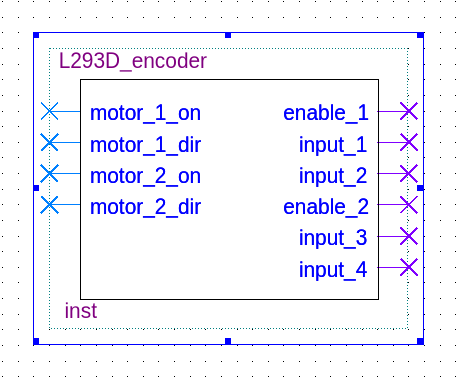
\includegraphics[width=.48\textwidth]{symbols/individual_placeholder.png}
  \caption{The block symbol of the (NAME) individual block used in the (NAME) functional unit.}
    \label{fig:individual-1-2-block}
\end{figure}
\begin{figure}[h]
  \centering
  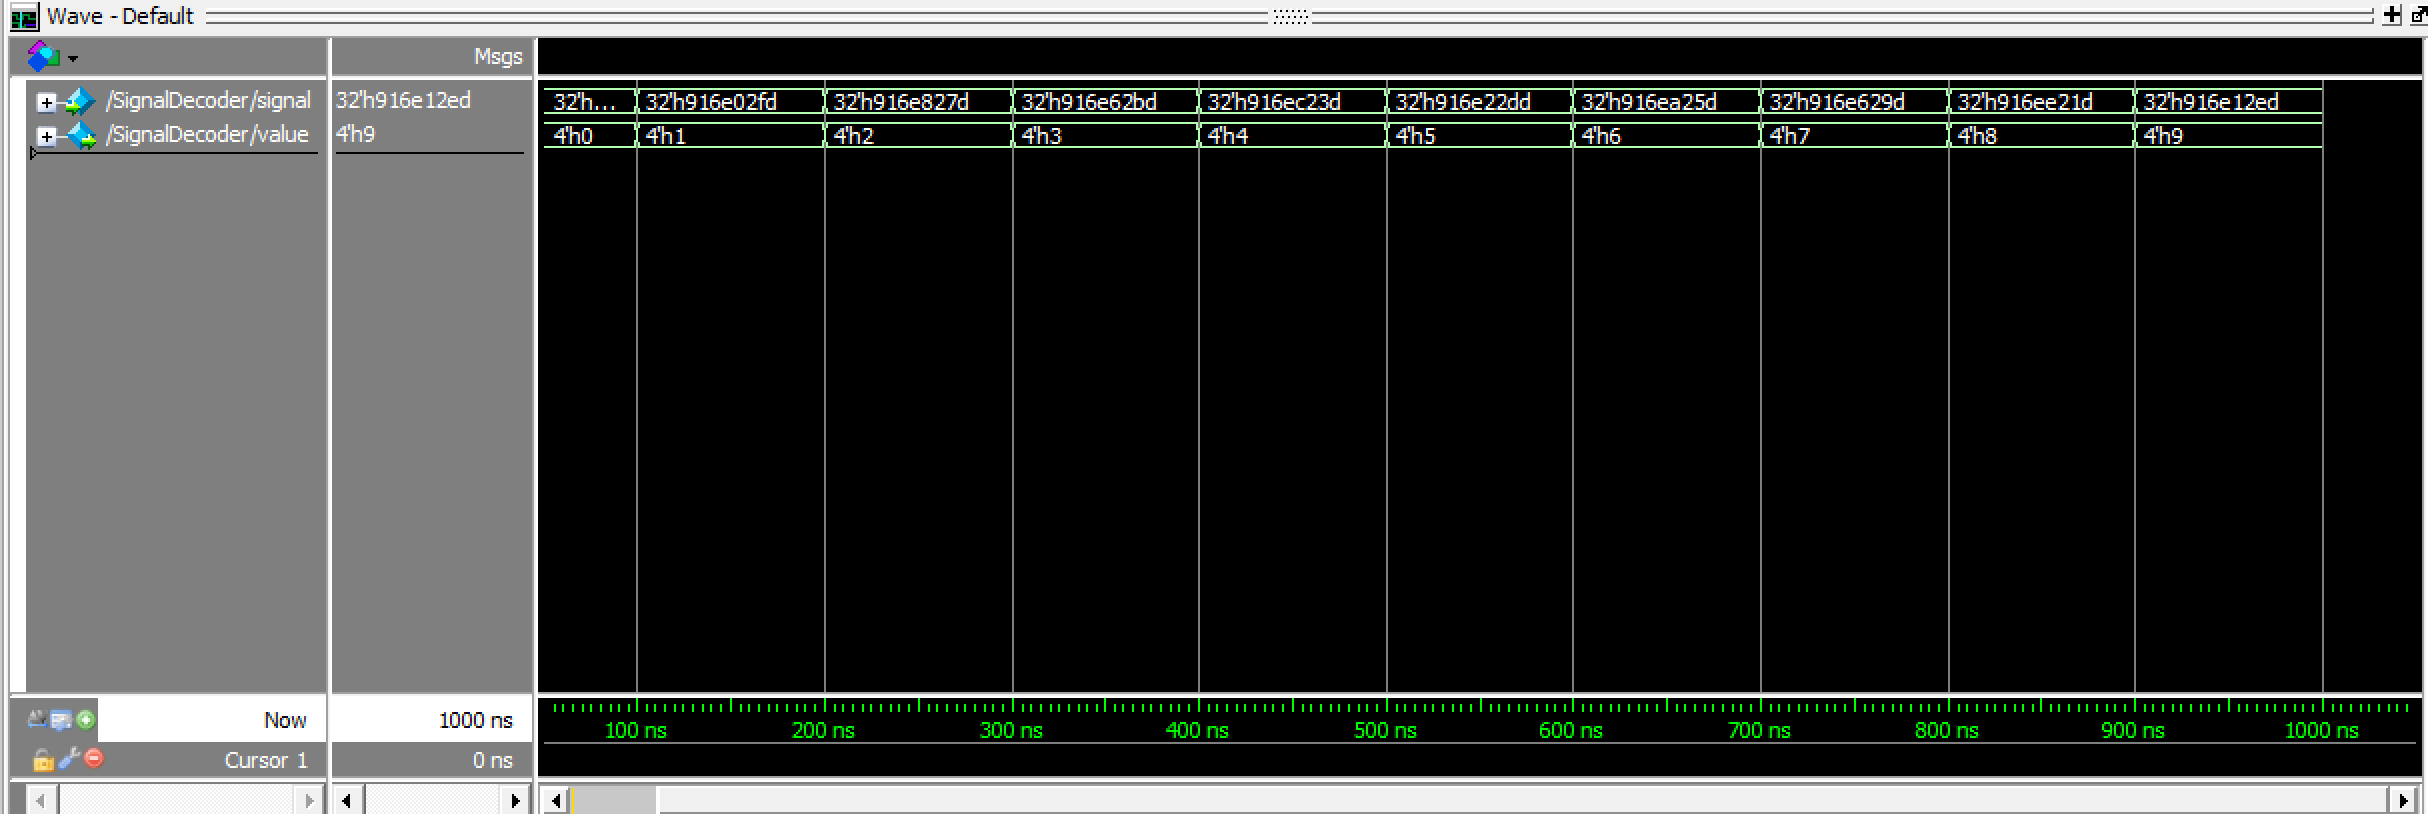
\includegraphics[width=.98\textwidth]{sims/vcr_testing/moduleTests/SignalDecoder/SignalDecoder_sim.png}
  \caption{The simulation results of the SignalDecoder individual block used in the vcr\_decoder functional unit.}
    \label{fig:individual-1-2-sim}
\end{figure}



\clearpage



\subsubsection{ShiftRegister Individual Block}
The ShiftRegister Individual Block is used to store the 32-bit IR signal value bit by bit as as it is read in by the ReadState Module. The input and output specifications follow, as well as the block diagram (\textbf{Figure C}), and simulation results \textbf{Figure D} for the individual block.
\begin{itemize}
  \item \textbf{Inputs:  } Inputs
  \item \textbf{Outputs: } Output
\end{itemize}
\begin{figure}[h]
  \centering
  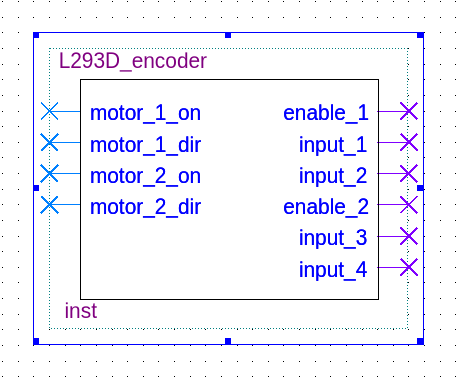
\includegraphics[width=.48\textwidth]{symbols/individual_placeholder.png}
  \caption{The block symbol of the ShiftRegister individual block used in the vcr\_decoder functional unit.}
    \label{fig:individual-1-2-block}
\end{figure}
\begin{figure}[h]
  \centering
  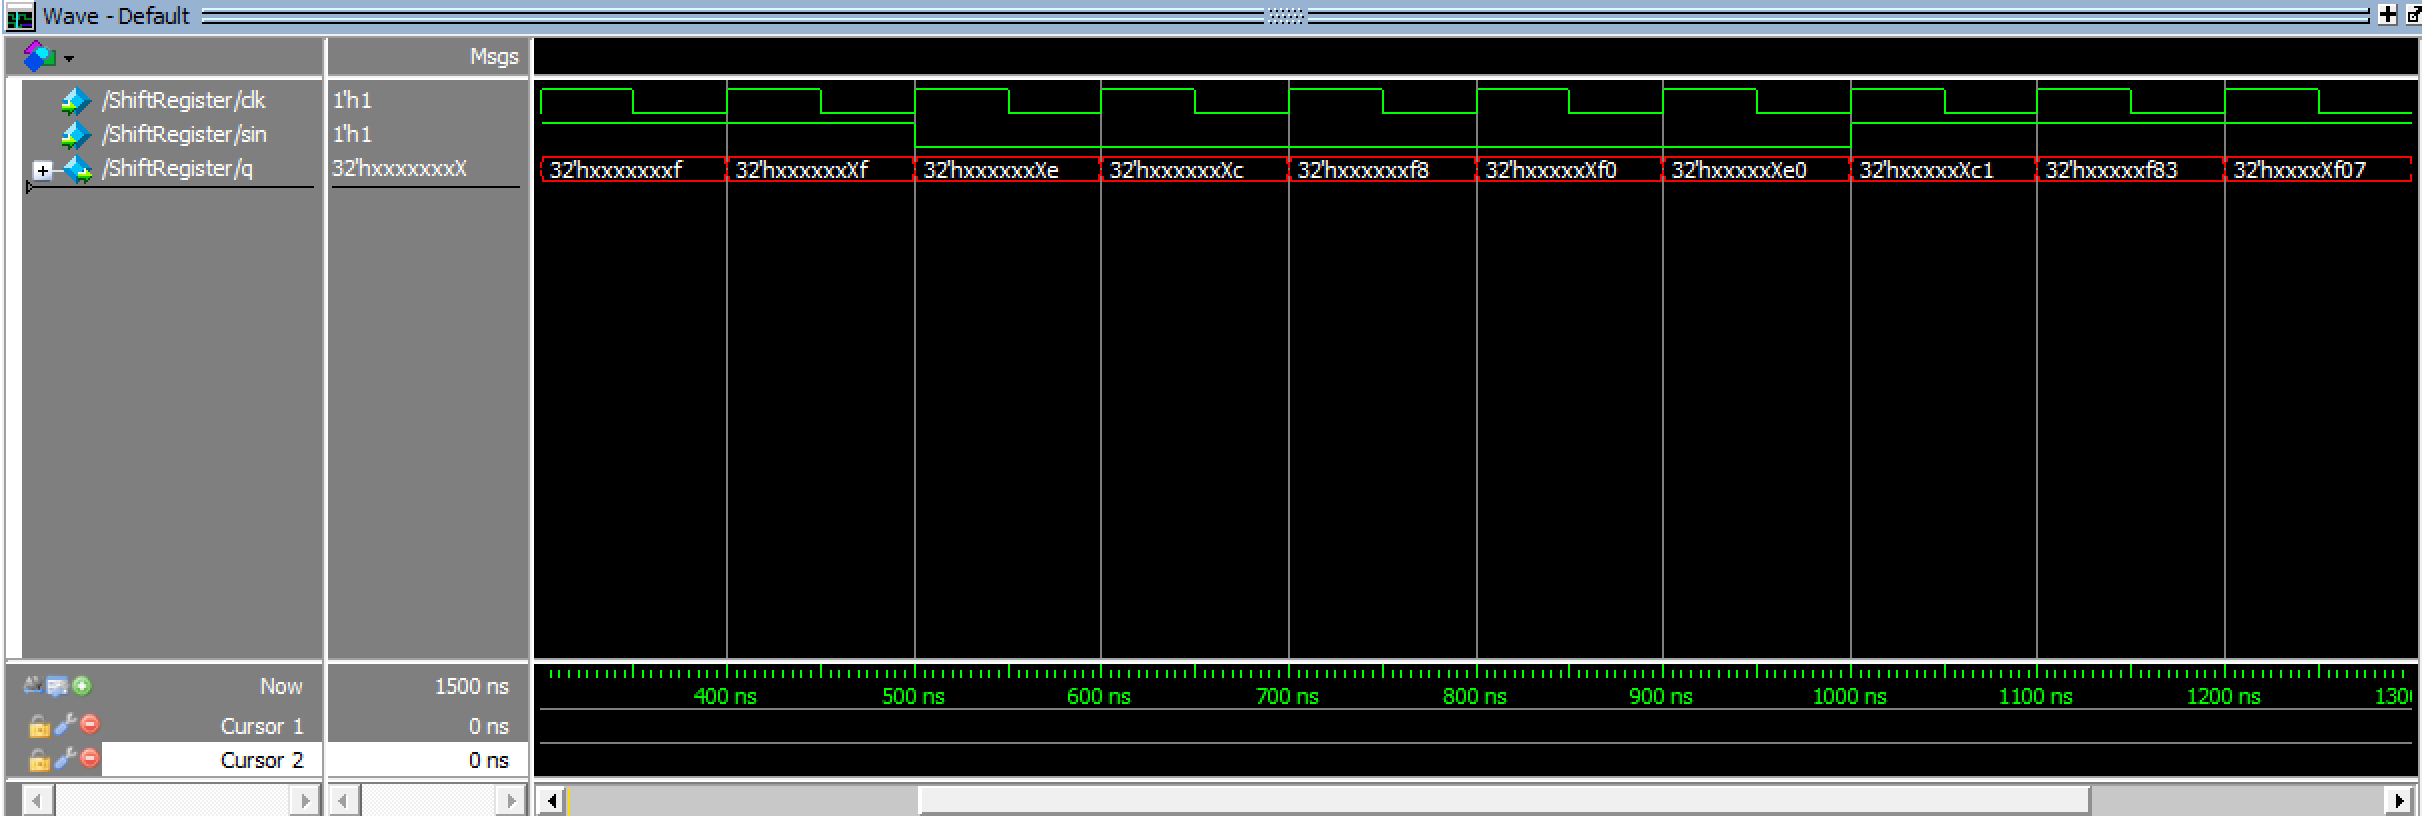
\includegraphics[width=.98\textwidth]{sims/vcr_testing/moduleTests/shiftRegister/ShiftRegister_sim.png}
  \caption{The simulation results of the ShiftRegister individual block used in the vcr\_decoder functional unit.}
    \label{fig:individual-1-2-sim}
\end{figure}



\clearpage



\appendix
\section{SystemVerilog Files}
This appendix will list the SystemVerilog code used for each block used in the design project.

GENERATE ME



\clearpage




\section{Simulation Files (Do Scripts)}
This appendix will list the Do Scripts used to simulate each block used in the design project.

GENERATE ME




\end{document}
